\documentclass[12pt, oneside]{book}
\usepackage[utf8]{inputenc}
%%%%%%%%%%%%%%%%%%%%%%%%%%%%%%%%%%%%%%%%%
% University Assignment Title Page 
% LaTeX Template
% Version 1.0 (27/12/12)
%
% This template has been downloaded from:
% http://www.LaTeXTemplates.com
%
% Original author:
% WikiBooks (http://en.wikibooks.org/wiki/LaTeX/Title_Creation)
%
% License:
% CC BY-NC-SA 3.0 (http://creativecommons.org/licenses/by-nc-sa/3.0/)
% 
%
%%%%%%%%%%%%%%%%%%%%%%%%%%%%%%%%%%%%%%%%%
%----------------------------------------------------------------------------------------
%	PACKAGES AND OTHER DOCUMENT CONFIGURATIONS
%----------------------------------------------------------------------------------------
\usepackage[a4paper,hmargin=2.8cm,vmargin=2.0cm,includeheadfoot]{geometry}
\usepackage{textpos}
%\usepackage{natbib} % for bibliography
\usepackage{tabularx,longtable,multirow,caption}%hangcaption
\usepackage{fancyhdr} % page layout
\usepackage{url} % URLs
\usepackage[english]{babel}
\usepackage{amsmath}
\usepackage{graphicx}
\usepackage{dsfont}
\usepackage{tocloft}
\usepackage{etoolbox}
\usepackage{titlesec}
\usepackage{csquotes}

\usepackage{epstopdf} % automatically replace .eps with .pdf in graphics
%\usepackage{backref} % needed for citations
\usepackage{array}
\usepackage{latexsym}


\usepackage[pdftex,hypertexnames=false,colorlinks]{hyperref} % provide links in pdf

\usepackage{blindtext} %fake text
\usepackage[sorting = none]{biblatex} %bibliography
\usepackage{siunitx}
\usepackage{subcaption}
\usepackage{cleveref}
\usepackage{pstricks,pstricks-add}
\usepackage{dialogue}
\usepackage{enumitem}
\usepackage{algorithmicx}
\usepackage{booktabs}
\usepackage{ragged2e}
\usepackage{tabularx}
\usepackage{glossaries}
\usepackage{verbatim}
\usepackage{float}



% For brackets
\newcommand\BrText[2]{%
  \par\smallskip
   \noindent\makebox[\textwidth][r]{$\text{#1}\left\{
    \begin{minipage}{\textwidth}
    #2
    \end{minipage}
  \right.\nulldelimiterspace=0pt$}\smallskip
}

\newcommand*{\myrulefill}[3][]{%
  \makebox[#2]{#1%
    \leaders\hrule height \dimexpr.5ex+.2pt\relax depth \dimexpr -.5ex+.2pt\relax \hfill% Left rule
    \enskip{#3}\enskip% Text (and surrounding spaces)
    \leaders\hrule height \dimexpr.5ex+.2pt\relax depth \dimexpr -.5ex+.2pt\relax \hfill\kern0pt}% Right rule
}
\makeglossaries
\newacronym{lccrf}{LCCRF}{Linear Chain Conditional Random Field}


\newglossaryentry{nlp}
{
        name=NLP,
        description={Natural Language Processing. The field of computational linguistics concerned with allowing computers to process and analyse natural (human) language data, specifically tasks that require the programme to ``understand" the text in some way},
        first = {Natural Language Processing (NLP)},
        long = {Natural Language Processing}
}

\newglossaryentry{crf}
{
        name=CRF,
        description={Conditional Random Field. A graph-based modelling technique that classifies sequences of tags given a sequence of inputs.},
        first = {Conditional Random Field (CRF)},
        long = {Conditional Random Field},
        plural = {CRFs},
        firstplural = {Conditional Random Fields (CRFs)},
}

\newglossaryentry{ml}
{
        name=ML,
        description={Machine Learning. The area of computer science concerned with learning the behaviour of a computer by examples instead of implementation by a programmer.},
        first = {Machine Learning (ML)},
        long = {Machine Learning}
}

\newglossaryentry{ca}
{
        name=CA,
        description={Conversation Analysis. A sub-field of linguistics concerned with the study of conversations.},
        first = {Conversation Analysis (CA)},
        long = {Conversation Analysis}
}

\newglossaryentry{lstm}
{
        name=LSTM,
        description={Long short term memory. A type of RNN architecture},
        first = {Long Short Term Memory (LSTM)},
        long = {Long Short Term Memory}
}

\newglossaryentry{geek}
{
        name=GEEK,
        description={Graph of Embedded Extracted Keyphrases. Our novel topic extraction algorithm},
        first = {Graph of Embedded Extracted Keyphrases (GEEK)},
        long = {Graph of Embedded Extracted Keyphrases}
}

\newglossaryentry{gru}
{
        name=GRU,
        description={Gated Recurrent Unit. A type of RNN architecture},
        first = {Gated Recurrent Unit (GRU)},
        long = {Gated Recurrent Unit}
}


\newglossaryentry{rnn}
{
        name=RNN,
        description={Recurrent Neural Network. Neural networks that can process sequences of varying length by passing a state of numbers from the first to the last neuron in the layer, modifying the state in a way depending on the input at the corresponding position within the sequence},
        first = {Recurrent Neural Network (RNN)},
        long = {Recurrent Neural Network},
        plural = {RNNs},
        firstplural = {Recurrent Neural Networks (RNNs)},
}

\newglossaryentry{nn}
{
        name=NN,
        description={(Artificial) Neural Network. A very flexible function (loosely based on the neurons of human brains) whose behaviour is specified by a set of parameters. A type of machine learning model},
        first = {Neural Network (NN)},
        long = {Neural Network},
        plural = {NNs},
        firstplural = {Neural Networks (NNs)},
}

\newglossaryentry{swda}
{
        name=SwDA,
        description={Switchboard Dialogue Act. The name of a dataset of phone conversations held via the Switchboard helpline telephone service annotated with dialogue acts by humans},
        first = {Switchboard Dialogue Act (SwDA)},
        long = {Switchboard Dialogue Act},
}

\newglossaryentry{lda}
{
        name=LDA,
        description={Latent Dirichlet Allocation. A topic model that assumes text is generated by repeatedly sampling a distribution of topics and then sampling that topic for a word.},
        first = {Latent Dirichlet Allocation (LDA)},
        long = {Latent Dirichlet Allocation},
}

\newglossaryentry{da}
{
        name=DA,
        description={Dialogue Act. The intended social action of an utterance. E.g. the intended social action of the utterance ``Hello" is a greeting},
        first = {Dialogue Act (DA)},
        long = {Dialogue Act},
        plural = {DAs},
        firstplural = {Dialogue Acts (DAs)},
}

\newglossaryentry{pca}
{
        name=PCA,
        description={Principal Component Analysis. A dimensionality reduction technique that determines convenient basis vectors and maps data onto these basis vectors.},
        first = {Principal Component Analysis (PCA)},
        long = {Principal Component Analysis},
}

\newglossaryentry{pos}
{
        name=PoS,
        description={Part of Speech. The grammatical function a word serves, e.g. ``house" $\rightarrow$ noun},
        first = {Part of Speech (PoS)},
        long = {Part of Speech},
}

\newglossaryentry{ner}
{
        name=NER,
        description={Named Entity Recognition. Identifying named entities, such as ``Donald Trump", ``CIA" or, ``Coca-Cola" automatically},
        first = {Part of Speech (PoS)},
        long = {Part of Speech},
}


\newglossaryentry{embedding}{
    name=embedding,
    description={A vector representing the meaning of a word or of a sequence of words}
    }

\newglossaryentry{model}{
    name=model,
    description={A function mapping inputs to outputs whose behaviour is statistically learned given a set of training data}
    }
    
\newglossaryentry{neuron}{
    name=neuron,
    description={An elementary information processing device that takes an input, and outputs a normalised weighted sum. The weights in the weighted sum determine its behaviour and are statistically learned. The atomic components of neural networks}
    }
    
\newglossaryentry{glove}{
    name=GloVe,
    description={\textbf{Glo}bal \textbf{Ve}ctors. A type of word embedding}
    }
    
\newglossaryentry{numberbatch}{
    name=ConceptNet Numberbatch,
    description={A type of word embedding}
    }

\newglossaryentry{utterance}{
    name=utterance,
    description={A section of spoken language that begins and ends with a pause from the speaker. In this work we approximate utterances as sentences}
    }
    
\newglossaryentry{keyphrase}{
    name=key-phrase,
    description={Single or multi-word expressions that represent the topics of a text}
    }

%WORD COUNT STUFF
\newcommand{\detailtexcount}[1]{%
  \immediate\write18{texcount -merge -sum -q #1.tex output.bbl > #1.wcdetail }%
  \verbatiminput{#1.wcdetail}%
}

\newcommand{\quickwordcount}[1]{%
  \immediate\write18{texcount -1 -sum -merge -q #1.tex output.bbl > #1-words.sum }%
  \input{#1-words.sum} words%
}

\newcommand{\quickcharcount}[1]{%
  \immediate\write18{texcount -1 -sum -merge -char -q #1.tex output.bbl > #1-chars.sum }%
  \input{#1-chars.sum} characters (not including spaces)%
}

% FIgure space
%\renewcommand{\topfraction}{.85}
%\renewcommand{\bottomfraction}{.7}
%\renewcommand{\textfraction}{0.15}
%\renewcommand{\floatpagefraction}{.9}
%\renewcommand{\dbltopfraction}{.66}
%\renewcommand{\dblfloatpagefraction}{.66}


\graphicspath{ {figures/} }
\addbibresource{bibliography.bib}
\renewcommand{\baselinestretch}{1.1}

%====================================SETUP===============================================

\setcounter{tocdepth}{1} % supress subsections from content
%\fancyhead{}

\newcommand{\changefont}{%
    \fontsize{11}{12}\selectfont
}
%\fancyhead[L]{\fontsize{10}{12}}

\fancyhead[R]{\changefont \slshape \rightmark} %section
\fancyhead[L]{\changefont \slshape \leftmark} %chapter

\hypersetup{%
  colorlinks = true,
  linkcolor  = black
}

\setlength{\cftbeforetoctitleskip}{-40pt}
\setlength{\cftaftertoctitleskip}{0pt} % make content fit on one page

\titleformat{\chapter}[display]
    {\normalfont\huge\bfseries}{\chaptertitlename\ \thechapter}{20pt}{\Huge}
\titlespacing*{\chapter}{0pt}{0pt}{40pt}

 %make chapters not start a new page
\makeatletter

\renewcommand\chapter{%
%   \if@openright\cleardoublepage\else\clearpage\fi
  \vfil \penalty+9000 \vfilneg
% Something from the following two lines could be retained:
%   \thispagestyle{plain}%
%   \global\@topnum\z@
  \@afterindentfalse
  \secdef\@chapter\@schapter
}

\patchcmd{\@makeschapterhead}{\vspace*{50\p@}}{\vspace*{-20\p@}}{}{}%


\makeatother

%\setglossarypreamble{\vspace*{-\baselineskip}}

%========================================================================================
\begin{document}

%TC:ignore
%\quickwordcount{main}
%\quickcharcount{main}
%\detailtexcount{main}
%TC:endignore

\renewcommand{\headrulewidth}{0pt}% Remove header rule
\pagestyle{plain}
%TC:ignore
\begin{titlepage}

\newcommand{\HRule}{\rule{\linewidth}{0.5mm}} % Defines a new command for the horizontal lines, change thickness here


%----------------------------------------------------------------------------------------
%	LOGO SECTION
%----------------------------------------------------------------------------------------


\includegraphics[width = 5cm]{imperial.pdf}\\[0.5cm] 

\center % Center remainder of the page

%----------------------------------------------------------------------------------------
%	HEADING SECTIONS
%----------------------------------------------------------------------------------------

\textsc{\Large Imperial College London}\\[0.5cm] 
\textsc{\large Department of Physics}\\[0.5cm] 

%----------------------------------------------------------------------------------------
%	TITLE SECTION
%----------------------------------------------------------------------------------------

\HRule \\[0.4cm]
{ \huge \bfseries The Structure of Conversation}\\ % Title of your document
\HRule \\[1.5cm]
 
%----------------------------------------------------------------------------------------
%	AUTHOR SECTION
%----------------------------------------------------------------------------------------

\begin{minipage}{0.4\textwidth}
\begin{flushleft} \large
\emph{Author:}\\
Jonas Scholz
\end{flushleft}
\end{minipage}
~
\begin{minipage}{0.4\textwidth}
\begin{flushright} \large
\emph{Supervisor:} \\
Tim Evans
\end{flushright}
\end{minipage}\\[4cm]


%----------------------------------------------------------------------------------------
%	FOOTER & DATE SECTION
%----------------------------------------------------------------------------------------
\vfill % Fill the rest of the page with whitespace

\end{titlepage}


%TC:endignore
\chapter*{Abstract}
\thispagestyle{empty}
We evaluate, improve and modernise existing \gls{nlp} methods and adapt them specifically for conversations between 2 or more individuals. Concretely, we improve methods for \textbf{\gls{da} classification} and \textbf{topic extraction}.

In \gls{da} classification, the aim is to automatically map sentences in conversations to their appropriate social function, such as ``Hello" $\rightarrow$ greeting. we re-implement, fix, tweak, and modernise an existing classifier by IBM Research\cite{kumar2017dialogue} to achieve state of the art performance in the \gls{swda} corpus \cite{swda}, which is commonly used for the evaluation of \gls{da} classifiers.
Our \gls{model} achieves an accuracy of $\mathbf{84.6 \pm 0.3}$, outperforming the previous state of the art \gls{model} (83.1\%)\cite{ravi2018self} and even the inter-annotator accuracy between the human annotators who created the \gls{swda} dataset\cite{swda} (84\%).

Our second focus is topic extraction, in which the goal is to identify \textit{which} topics are featured within a conversation and \textit{at what times} (topic labelling and segmentation respectively). We evaluate a large number of existing approaches and identify their limitations when applied to casual conversations to create a novel topic extraction algorithm.
%, which outperforms the state of the art topic segmentation \gls{model} BayesSeg.
Using the standard metric for evaluating topic segmentation, windowDiff, $w_d$, (in which a lower score indicates a better segmentation performance) our algorithm achieves $w_d = \mathbf{0.22 \pm 0.04}$, outperforming previous state of the art BayesSeg\cite{eisenstein2008bayesian} which achieved $w_d = 0.39 \pm 0.06$ when applied to the same conversation transcripts.

Finally, we apply the improved methods to 18,000 conversations from the Spotify podcast dataset\cite{clifton-2020100000} to create and publish a corpus of conversations annotated with linguistic features, enabling future large-scale conversation analysis.

\begin{figure}
    \centering
    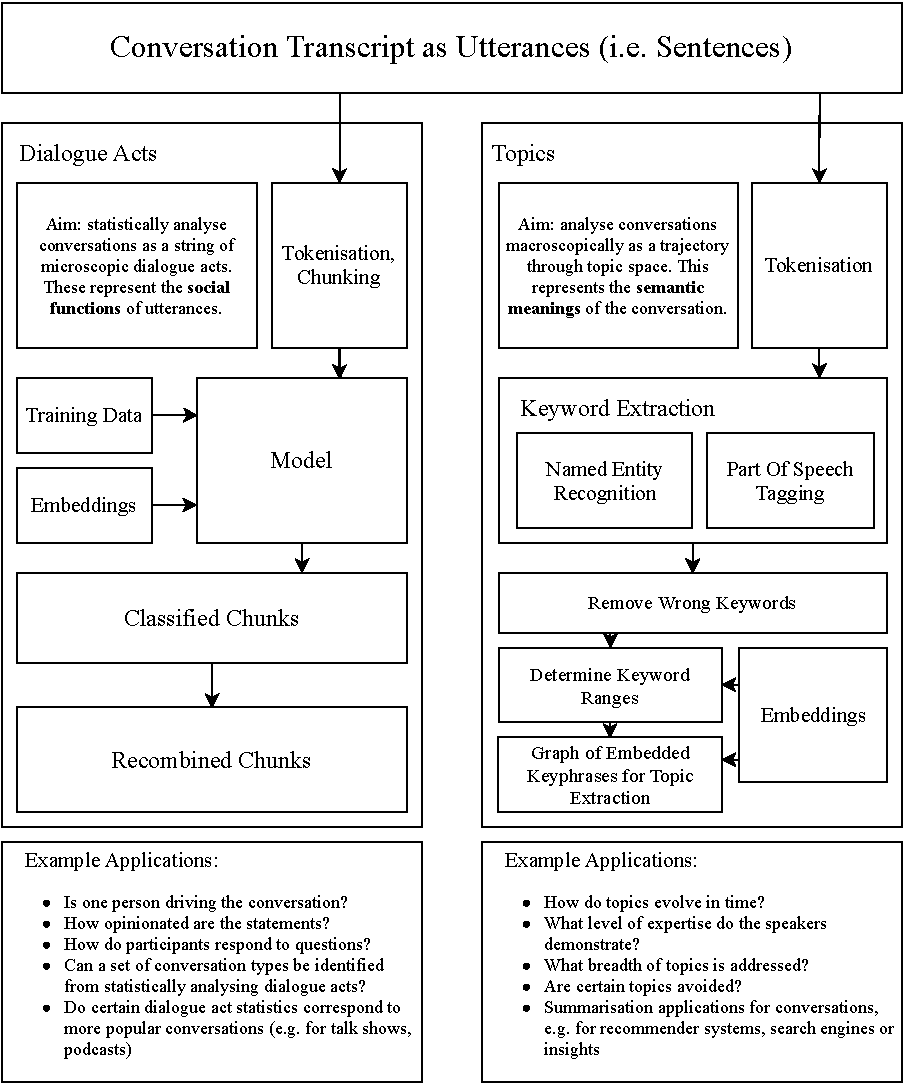
\includegraphics{overview.pdf}
    \caption{Overview of our final methods.}
    \label{fig:overview}
\end{figure}
\glsresetall
\newpage


%TC:ignore
\tableofcontents
\thispagestyle{empty}
\printglossaries

\pagestyle{fancy}
%644 too many words in wordcount

%TC:endignore
\newpage
\renewcommand{\headrulewidth}{0.5pt}% Re-enable header rule
\chapter{Introduction}

%\subsubsection{The Development of Natural Language Processing}
The rapid developments within the field of \gls{nlp} over the last decade and the exponential advances in computational performance\cite{mooresLaw} have made automated text analysis freely available and economical to use. \Gls{nlp} has since found wide commercial application, from sentiment analysis to gauge customer reviews or the optimism in financial markets\cite{sentimentReview} to virtual assistants, such as the Google assistant, Apple's Siri or Amazon's Alexa\cite{virtualAssistants}.

While many applications were developed for commercial use, their implementations are often (relatively) simple to recreate using mature libraries such as Google's TensorFlow\cite{abadi2016tensorflow} or Facebook's PyTorch\cite{paszke2019pytorch}. This has allowed independent researchers to apply \gls{nlp} to a vast number of areas, such as the analysis of tweets to appropriately respond to mass emergencies (such as earthquakes)\cite{twitterEmergencies}, or the analysis of newspaper articles to identify media bias\cite{mediaBias}.

\subsubsection{NLP for Conversation Analysis}
Within the linguistic field of \gls{ca}, the use of \gls{nlp} is more limited. 
Most existing research is not automated and requires researchers to manually annotate conversations with the linguistic features they are investigating, which is a time consuming and unrewarding process and severely limits the \textit{amount} of text that researchers can analyse. It also means that uncertainties are difficult to estimate as the researchers have to either estimate their own error rates in annotating the text, use multiple annotators to gain quantitative inter-annotator accuracies or not report uncertainties at all --- non of which are ideal options.

\subsubsection{Conversation Analysis at Scale}
Initially, we aimed to begin filling the gap of using \gls{nlp} for conversation analysis, by applying existing \gls{nlp} methods to a large corpus of conversations held on podcasts from the public Spotify Podcast dataset\cite{clifton-2020100000} and analysing it statistically to gain insights into specific questions around conversation structure, such as \textit{what makes conversations interesting to an audience?} Specifically we wanted to investigate the (macroscopic) evolution of topics within a conversation and the (microscopic) structure of sentences and their responses by conversation members. Unfortunately, conversations are noisy: conversation members talk over each other, struggle to find the right words, use humour, sarcasm, slang, and analogies and as we evaluated existing \gls{nlp} methods, we found they were ill-equipped to deal with that fact (especially the \gls{nlp} tools used for modelling topics).

\subsubsection{Improving and Adapting NLP for Conversations}
Because of the disappointing performance of the \gls{nlp} methods we tested, we decided to shift our intentions from \textit{analysing conversations} using existing \gls{nlp} methods to \textit{improving} said methods and adapting them to conversations. We address two separate \gls{nlp} methods: \gls{da} classification and topic extraction.

Specifically, to improve methods of \gls{da} classification (which we define in Sec. \ref{ssec: DAs}), we re-implement an existing language \gls{model} designed by a team at IBM Research\cite{kumar2017dialogue}, fix a bug, tweak it and modernise it to achieve state of the art performance.

Secondly, within the topic extraction area, we hand-annotate conversation transcripts as a baseline for evaluation, quantify the performance of existing methods, identify key issues, and create a novel topic extraction algorithm that is more robust against said key issues.

\subsubsection{An Annotated Corpus of Conversations}
Finally, to enable future research into the linguistic questions we \textit{initially} aimed to answer, we annotate 18,000 conversation transcripts from the Spotify podcast dataset\cite{clifton-2020100000} with both topics and \glspl{da} using the methods we develop and publish it.

\subsubsection{Applications}
The applications of the algorithms we develop and improve in this thesis are numerous. Commercially, they can be used to make group meetings more productive by automating meeting minutes and summarising meetings, or by analysing the process of arriving at conclusions\cite{daApplications}, they can make interviewers, podcast hosts, and talk-show hosts more aware of what microscopic behaviours and which general topics lead to greater interest or they can improve the behaviour of the aforementioned virtual assistants by determining what the user wants\cite{daApplications}. Medically, some linguistic features that we automatically extract can be used to help diagnose mental illnesses such as social anxiety and depression\cite{ap_psychological}. 
Within linguistics, the methods we improve can be applied for blue skies research e.g. of the speech patterns of politicians\cite{ap_trump} or the evaluation of movie dialogues\cite{movieDialogue}. \newline



%\subsubsection{The Intersection of Conversation Analysis and Natural Language Processing}
%Our project is at the intersection of \gls{ca} and \gls{nlp}, as we attempt to use \gls{nlp} to do \gls{ca}.

%Initially, we wanted to apply \gls{nlp} methods to a large number of conversations to statistically determine what we call the \textit{bounds of conversation}, i.e. the things that all conversations have in common. We quickly found that the techniques commonly used in \gls{nlp} were not very effective when dealing with conversations, so we decided to shift the focus of this project to the improvement of existing \gls{nlp} techniques.

%\section{Which Conversations?}
    \subsection{Spotify Podcast Corpus \label{ssec: spotify corpus}}
        Conversation podcasts are a type of podcast in which the host invites one or more guests for a recorded conversation. The format is similar to a traditional talk-show, but conversations are usually longer (from 0.5-4 hours long), more in-depth, and follow a less rigid structure.  The recorded conversation is then published on streaming platforms such as YouTube or Spotify, where the audience can listen to it.
        
        The Spotify podcast corpus\cite{clifton-2020100000} is a collection of 100,000 episodes from different podcast shows hosted on Spotify and our primary source of conversations. It features over 50,000 hours of audio and 600 million words spoken in a large number of shows that feature a number of conversation lengths, topics, styles and qualities. The corpus provides audio files as well as podcast transcripts automatically transcribed by Google's speech to text service. The quality of these transcriptions varies heavily between topics discussed, microphone quality and clarity of the conversations and are a key limitation for our work.
        
    \subsection{Switchboard Dialogue Act Corpus \label{ssec: swda}}
        A secondary source of conversations is provided by the \gls{swda} corpus, a collection of 1155 five-minute conversations between two participants, in which callers question receivers on pre-determined topics such as child care, recycling and new media.\cite{fang2012annotation}. It is transcribed by humans, annotated with \glspl{da} (see Sec. \ref{ssec: DAs}) as well as the pre-determined topic of the conversation.
        %Besides being used as training data for some of the models we train, the \gls{swda} corpus provides us with a different type of conversation that we can analyse: short, private, topical phone conversations instead of in-depth conversations primarily recorded for an audience.
\glsresetall % 400 words
\chapter{Background \label{cpt: background}}

Our analysis is based on concepts from the \gls{ca}, a sub-field of linguistics, and is automated using tools and techniques from the \gls{nlp} area of computer science. This chapter first introduces all the \gls{nlp} concepts and tools used within this work (Sec. \ref{sec: nlp} to \ref{ssec: word embeddings}) and then all the linguistic concepts that our analysis is built on (Sec. \ref{sec: ca})
%and finally introduces work directly related to our project (Sec. ???).

\section{An Overview of Natural Language Processing \label{sec: nlp}}

Natural Language Processing (NLP) is a sub-field of computer science, artificial intelligence and linguistics, which attempts to use computers to analyse natural (human) language data. An example of advanced NLP applications are \textit{virtual assistants} such as the \textit{Google Home} or \textit{Amazon Alexa} devices, which need to understand queries spoken by a human (speech recognition), understand them (natural language understanding), execute the functionality that was asked for and formulate a response (natural language generation). The methods we apply fall firmly within the area of natural language understanding, as we apply (and modify) commonly used methods to the largely unexplored landscape of human conversations.

%NLP has had an increasingly important role and is commonly referenced as a key component to an \textit{artificial general intelligence} (AGI). CITE TURING.

Most NLP applications deal with low-noise text data, such as news articles, product reviews, or direct queries. Conversations between humans do not fall within this category and are associated with large amounts of noise: from members of the conversation talking over one-another to the use of sarcasm, jokes or slang, conversations are messy. For this reason, conversation analysis has largely been manual in nature. 
\section{Machine Learning \label{sec: ML}}
    A traditional computer programme takes some inputs $X$, does something with those inputs and outputs some output $Y$. It can be thought of as a function $f: X \rightarrow Y$. The behaviour of that function $f$ is defined by the programmer.
    %, who specifies what the computer is supposed to do with $X$ to turn it into $Y$.

    %The objective of \gls{ml} is to \textit{learn} the behaviour of such a function $f$ statistically as $\hat{f}$.
    In \gls{ml}, the behaviour of $\hat{f}$ is not implemented by a programmer, but statistically learned from data. $\hat{f}$ is called the \textbf{\gls{model}}. In practice, $\hat{f} = \hat{f}_\theta$ is highly flexible and its behaviour specified by a set of parameters $\theta$. These parameters are initially randomly assigned and then automatically tweaked until $\hat{f}_\theta$ shows the desired behaviour in a process called training (see Sec. \ref{ssec: training}).

    \gls{ml} is useful in cases that have too many inputs to be implemented traditionally, such as image recognition or \gls{nlp}.

    \subsection{Supervised Learning}
        In supervised learning, the \gls{ml} algorithm is fed pairs $(X, Y)$ of inputs $X$ and matching outputs $Y$ that were labelled manually by humans. If, for example, one wanted to train a \gls{model} that recognises cats, $X$ would be an image of a cat or an image not of a cat, and $Y$ would be the corresponding label \textit{cat} or \textit{not cat}. The algorithm uses $(X, Y)$ to iteratively compare its own prediction $\hat{f}_\theta(X) = \hat{Y}$ to the true output $Y$ and slightly adjusts its parameters $\theta$ to match that true output. This process is called training and the pairs of $(X, Y)$ accordingly are called training data. %There are many different approaches and implementations of the functions $\hat{f}_\theta$ and the training process. The type of $\hat{f}_\theta$ we use is called a \gls{nn} and it is trained through a process called backpropagation. We expand on this in section ???.
        Supervised learning is the main flavour of \gls{ml} used for this project.

    %\subsection{Unsupervised Learning}
        %In unsupervised learning, only the input data $X$ is provided (and no true labels $Y$). The \gls{ml} algorithm then uses some statistical techniques to provide some useful insights. The two main uses of unsupervised learning in this project are \gls{pca}, which reduces high-dimensional data to lower-dimensional data while trying to preserve similarity, and cluster analysis, which finds similarities within the datapoints $X$ and groups similar data-points together.
 
\section{Artificial Neural Networks \label{sec: neural nets}}

    \begin{figure}[h]
        \centering
        \begin{subfigure}[b]{0.9\textwidth}
            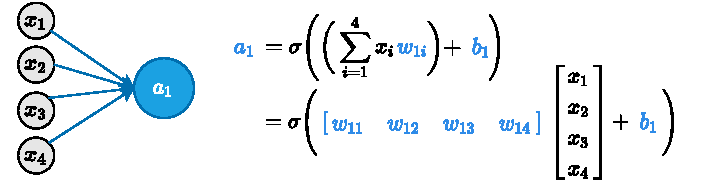
\includegraphics[width=\textwidth]{one_neuron.pdf}
            \caption{A single neuron connected to the input layer of 4 input neurons. It computes the activation function of the weighted sum of the previous layer's outputs as its own output. \label{subfig: neuron}}
        \end{subfigure}
        \hfill
        \begin{subfigure}[b]{0.9\textwidth}
            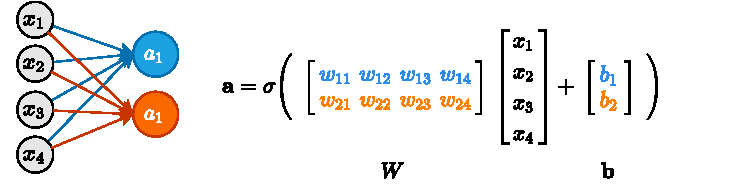
\includegraphics[width=\textwidth]{two_neurons.pdf}
            \caption{Using notation from linear algebra, the calculations computed by the whole layer (of two neurons) can be written as an activation function of a matrix multiplication and vector addition. \label{subfig: layer}}
        \end{subfigure}
        \caption{4 input neurons $x_i$ are connected to the next layer consisting of one neuron (a) or two neurons (b).}
    \end{figure}

    

    The models used for supervised learning throughout this project are called (artificial) neural networks (NNs). They are flexible information processing architectures (loosely) inspired by the network of neurons in the brain. It is not strictly necessary to understand the functionality of NNs to understand the rest of the project, simply noting that NNs are flexible functions $\hat{f}_{\theta} : X \rightarrow Y$ that can be trained to process information in the desired way using labelled training data $(X, Y)$ is enough. A quick introduction is however included for completeness.
    
    \subsection{Neurons}
        NNs are a connection of connected nodes called neurons that are sequentially organised into a number of layers. Each neuron contains a set of weights $w_i$ and a set of biases $b_i$ with $i \in [0, N_{in}]$, where $N_{in}$ is the number of inputs to that neuron. A neuron takes inputs $a_i^{(j)}$ from the previous layer $j$ and calculates its output as a weighted sum normalised by a non-linear \textit{activation function} $\sigma$ (see Sec. \ref{ssec: activation function}):
    
        \begin{equation}
            \label{eq: feed forward}
            a^{(j + 1)} = \sigma\bigg(\big(\sum_{i = 0}^{N_{in}} w_i a_i^{(j)}\big) + b\bigg).
        \end{equation}
        
        This output is the input for all connected neurons in the next layer, hence it is equal to $a^{(j+1)}$. This process of processing information is called the forward pass of the NN. A simple example of a neuron is shown in Fig. \ref{subfig: neuron}.
    
    \subsection{Layers}
        NNs are composed of multiple layers of multiple neurons. In many NNs, every neuron in layer $j$ is connected to every neuron in the next layer $j + 1$. We assume that this is the general case within this section. This allows for the use of linear algebra notation to simplify what each layer does.
        
        Writing the input vector of layer $j$ as $\mathbf{a}^{(j)}$, the weight matrix, containing all the weights of a neuron (column) for all neurons in a layer (row) as $W$ and the vector of biases of all neurons in a layer as $\mathbf{b}$ allows us to write the forward pass through each layer as
        
        \begin{equation}
            \mathbf{a}^{(j + 1)} = \sigma(W\mathbf{a}^{(j)} + \mathbf{b}),
        \end{equation}
        
        as \[
            \sigma\bigg( \big(x_0, x_1, \dots x_n) \bigg) = \bigg( \sigma(x_0), \sigma(x_1) \dots \sigma(x_n)\bigg). %todo make col vec
        \]
        
        A simple example, with only two layers can be found in Fig. \ref{subfig: layer}. The inputs to the first layer are the inputs to $\hat{f}_\theta$, $X$. The output(s) of the last layer are the predicted results $\hat{Y}$. 
        
        The information processing of a neural net with $N$ layers can thus be written as the repeated nested application of a weighted sum normalised at every layer $j$ by some $\sigma^{(j)}$:
        
        \begin{align}
            \label{eq: nested NN}
            \hat{\mathbf{Y}} = \mathbf{a}^{(N - 1)} &= \sigma^{(N-1)}\bigg(W^{(N - 1)}\mathbf{a}^{(N - 2)} + \mathbf{b}^{(N-1)}\bigg) \\
            &= \sigma^{(N-1)}\bigg(
                W^{(N - 1)}\big( \dots (
                \sigma^{(0)} \big(
                    W^{(0)} (\mathbf{X})) + \mathbf{b}^{(0)}
                    \big) \dots
                \big) + \mathbf{b}^{(N-1)} \nonumber
            \bigg).
        \end{align}
        
        The weights $W$ and biases $\mathbf{b}$ determine how the inputs $\mathbf{X}$ are processed to the outputs $\mathbf{Y}$ and are the parameters $\theta$ of the model. By inspecting Eq. \ref{eq: nested NN} and noting that every $W$ is a potentially large matrix and every $\mathbf{b}$ a potentially large vector of parameters, it is clear that the number of parameters grows quickly with the complexity of the NN's architecture (i.e. its number of neurons, and number of input features $\mathbf{X}$). It is not uncommon that the number of parameters exceeds 10s of millions for complex models. The state of the art language model, known as GPT-3 uses 175 billion parameters \cite{gpt3}. The training process, in which all of these parameters are tuned is explained in Sec. \ref{ssec: training}.
        
        The scale of complex NNs is also the reason why it is beneficial to frame computations as linear algebra operations: A computer's GPU (graphical processing unit) is capable of processing large numbers of repeated calculations much faster than central processing units (CPUs), by computing all required values in parallel\cite{herlihy2012art}. 
        Linear algebra computations (such as matrix multiplications and vector additions) are examples where highly parallel computation can accelerate computations significantly, reducing the time needed to process data using NNs significantly.\cite{herlihy2012art}
        
        \subsection{Activation Functions \label{ssec: activation function}}
    
        There are a number of different choices for the activation function $\sigma$. Most activation functions normalise values to lie within some fixed interval $(a_{min}, a_{max})$, i.e.
        \begin{equation}
        \sigma : x \rightarrow y, \hspace{3em} x \in [-\infty, \infty], y \in (a_{min}, a_{max}).
        \end{equation}
        
        Examples for $\sigma$ include $\tanh{x}$, $1/(1 + e^{-x})$, or the Heaviside step-function, each of which is used for different purposes.
        
        The normalisation provided by the activation function means that a small number of neurons can not dominate the final outcomes too heavily (known as the ``exploding gradients problem"). The second effect of these functions is the non-linearity they introduce, allowing for non-linear models for non-linear problems.
        
    \subsection{Training \label{ssec: training}}
        To train the NN is to determine a set of parameters $\theta$ that make the model map $X \rightarrow \hat{Y}$ in such a way that matches the provided \textit{true labels} $Y$. This is approached as an optimization problem, where the quantity minimised is called the loss.
        
        \subsubsection{Loss Function}
            The loss function maps predicted labels and true labels to the so-called loss $L$: \[\mathcal{L} : \hat{Y}, Y \rightarrow L.\] It is a measure of goodness of fit between the model's predictions and the true labels. One commonly used example is the mean-squared-error as the loss function:
            \[
                \mathcal{L} = \frac{\sum_{i = 1}^{n}(y_i - \hat{y}_i)^2}{n}, \hspace{2em} y_1 \dots y_n \in Y.
            \]
            
            Since $\hat{Y}$ depends on $\theta$, $\mathcal{L} = \mathcal{L}(\theta)$. Since $\mathcal{L}$ and $\sigma$ are both differentiable functions, partial derivatives of $\mathcal{L}$ with respect to $\theta$ can be calculated. 
        
        \subsubsection{Gradient Descent}
            By computing the gradient of $\nabla_\theta \mathcal{L}$ with respect to $\theta$, and slowly moving all weights towards the minimum along this gradient, a set of weights that minimises the $\mathcal{L}$ (and thus optimises the prediction) can be found. Writing all parameters $\theta$ as a vector $\boldsymbol{\theta}$, this gradient descent process can be written succinctly as
            
            \begin{equation}
                \boldsymbol{\theta} \rightarrow \boldsymbol{\theta} - \alpha \nabla_\theta \mathcal{L}(\boldsymbol{\theta}),
            \end{equation}
            
            repeated until convergence, where $\alpha << 1$ is the learning rate, chosen manually. 
\section{Neural Networks for Text Analysis \label{sec: NNs for text}}
    There are two key issues with using NNs for text-analysis:
    
    \begin{enumerate}
    \item NNs require equal-length inputs, but words and sentences can have variable lengths.
    \item NNs require $x_i \in X$ to be numbers, not words, sentences or characters. A simple map such as $a \rightarrow 1, b \rightarrow 2 \dots$ is worthless also, because words are arbitrary choices and don't have inherent meaning.
    \end{enumerate}
    

    The first issue is addressed by recurrent neural networks, see Sec. \ref{ssec: RNNs}.
    The second issue is addressed by so-called word-embeddings (Sec. \ref{ssec: word embeddings}) which lie at the heart of our project and NLP in general. 
\section{Recurrent Neural Networks \label{ssec: RNNs}}

    \begin{figure}[t]
        \centering
        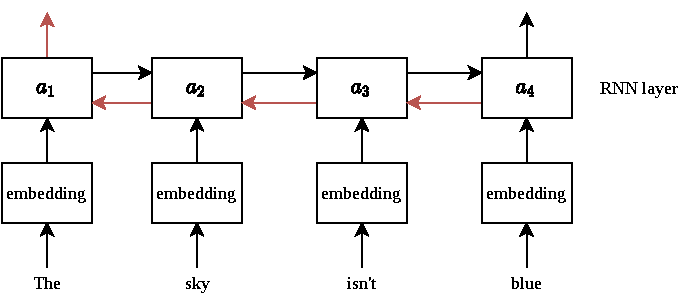
\includegraphics{rnn.pdf}
        \caption{The \gls{rnn} layer is given an input sequence of word \glspl{embedding}, calculates a hidden state depending on the first \gls{embedding} and the weights of the first neuron, and passes this hidden state on to the next \gls{neuron} within the \gls{rnn} layer. Every \gls{neuron} modifies the hidden state based on its weights and the input \gls{embedding} at its position and passes the modified state on. At the end of the sentence, the hidden state is passed on as the output of the layer. In a bidirectional \gls{model} (red arrows), a second hidden state is passed through the layer ``backwards".}
        \label{fig:rnn}
    \end{figure}
    Consider the following sentences as inputs to a \gls{nn}:

    \begin{table}[H]
    \begin{tabular}{|l|l|l|l|l|l|}
        \hline
        $i$   & 0   & 1   & 2     & 3    & 4    \\ \hline
        $s_1$ & The & sky & isn't & blue &      \\ \hline
        $s_2$ & The & sky & is    & blue &      \\ \hline
        $s_3$ & The & sky & is    & not  & blue \\ \hline
    \end{tabular}
    \centering
    \end{table}
    \noindent Using word \glspl{embedding} (see Sec. \ref{ssec: word embeddings}) we are able to turn these words into numbers that the \gls{nn} can process, but due to the (lack of) structure within sentences, we face another issue:
    Sentences $s_1$ and $s_2$ have different meanings, but because most words are the same, the inputs would appear relatively similar a hypothetical \gls{model} and yield similar outputs $\hat{Y}$. $s_1$ and $s_3$ have the same meaning, but are of different length. Therefore, in our hypothetical \gls{nn}, the inputs in positions $i = \{2, 3, 4\}$ are different, leading to potentially quite different outputs $\hat{Y}$.

    The problem is that in language, the absolute position of words within sentences is not particularly important, relative positions and context-words are: One word,``not", can change the meaning of the entire sentence dramatically.

     \Glspl{rnn} address these concerns and can process sequences of variable length such as sentences. \Glspl{rnn} use \glspl{neuron} as computational units in the same way traditional \glspl{nn} do, but instead of simply connecting \glspl{neuron} from the previous layer to \glspl{neuron} of the next layer, they connect \glspl{neuron} within a single layer, so that they form a directed graph. Every \gls{neuron} $n_i$ then corresponds to one entry in the sequence (e.g. one word in a sentence) and calculations are performed in a temporal direction: a hidden state of numbers is created at $n_1$, and repeatedly passed on to the next \gls{neuron} $n_{i+1}$, changed in a way determined by the $i+1$th entry and the \gls{neuron}'s parameters $\theta$ and passed on again. At the last \gls{neuron}, every entry has impacted the hidden state in some sensible way (specified by $\theta$) and the information can be passed to the next layer for further processing. A short example is given in Fig. \ref{fig:rnn}.


    \subsection{\gls{rnn} Architectures \label{ssec: rnn architectures}}
    The exact calculations that combine the hidden state with new inputs and parameters are determined by the internal structure of the \glspl{neuron}. The most prominently used \gls{neuron} architectures (which are also used in this project) are \gls{lstm}\cite{hochreiter1997long} and \gls{gru}\cite{chung2014empirical} architectures, both of which are capable of attaining state of the art performance on \gls{nlp} tasks\cite{huang2015bidirectional}.
    %%%%%%%%%%%%%%%%%%%

    \subsection{Bi-directional RNNs \label{ssec: bidirectional RNN}}
    If a \gls{rnn} layer is bi-directional, in addition to the hidden state being passed through the layer in a forward direction, another hidden state is passed through the layer backwards. This improves performance in many \gls{nlp} tasks, because e.g.  the impact of a given word on the meaning of a sentence does not only depend on its preceding, but also on its succeeding words. This means the \gls{rnn} layer has two outputs, one for the forwards pass and one for the backwards pass. This is indicated in red in Fig. \ref{fig:rnn}.

    \subsection{Outputting Hidden States \label{ssec: outputting hidden states}}
    In some cases, it is useful for the \gls{rnn} to have one output for every element in the sequence, not just one output at the end of the sequence. The different elements of the sequence still impact eachother's output, but now the output is a sequence of length equal to the input sequence. In that case, the hidden states of every \gls{neuron} are simply output to the next layer\cite{mlTextbook}.

    \subsubsection{When to Output Hidden States?}
    %Consider for example the following two different \glspl{model}, each with a different goal, but both taking a sequence of words $\mathcal{S}$ as an input.

    %The first \gls{model},
    %\begin{equation}
    %    \hat{f}_{\text{pos}}: \mathcal{S} \rightarrow \mathcal{P},
    %\end{equation}
    %outputs a sequence of \gls{pos} tags $\mathcal{P}$, one for every word e.g.
    %    \begin{equation*}
    %    \text{[The, house, is, green] $\rightarrow$ [article, %noun, verb, adjective]}.
    %    \end{equation*}
    %We still want the words to affect eachother's tags (i.e. green could be an adjective or a noun, depending on the other words in the sentence), but we want one tag for every word in the sequence. We want to map $N$ words $ \rightarrow N$ tags. In this case we want to return the $N$ hidden states as outputs.

    %The second \gls{model},
    %\begin{equation}
    %    \hat{f}_{q\Bar{q}}: \mathcal{S} \rightarrow q,
    %\end{equation}
    %outputs whether or not the sequence of words was a question or not, $q$. E.g.
    %    \begin{align*}
    %    \text{[The, house, is, green]} &\rightarrow \text{not a %question}\\
    %    \text{[Is, the, house, green]} &\rightarrow \text{question}.
    %    \end{align*}
    %It maps $N$ words $\rightarrow 1$ tag. In this case we want to output only one value, encapsulating the entire sequence; only the last \gls{neuron}'s value is returned.
    When we are mapping a sequence of length $N$ to a single tag (many to one) we only return the hidden state of the final \gls{neuron} encapsulating the entire sequence. When we instead map a sequence of length $N$ to an output sequence of tags of length $N$ instead, we return all hidden states.
 
\section[Conditional Random Fields]{Hidden Markov Models and Conditional Random Fields}

\Glspl{crf}\cite{originalCRF} are a graph-based modelling technique also used in sequence tagging commonly used in conjunction with \glspl{rnn} to improve classification accuracy. They can be understood as extensions to hidden Markov models.

\subsection{Hidden Markov Models}

    Hidden Markov models (HMMs) are based on markov processes. Markov processes describe a sequence of possible events in which the probability of each event depends \textit{only} on the state attained in the \textit{previous event}\cite{gagniuc2017markov}.
    HMMs consist of two such Markov processes: one process $\mathcal{X}$ with states that can be observed, such as a sequence of words, and one hidden process $\mathcal{Y}$ that depend on $\mathcal{X}$. The goal is to learn about $\mathcal{Y}$ by observing $\mathcal{X}$. HMMs use Bayesian modelling and apply them to Markov processes to make predictions\cite{klinger2007classical}.
   
   %TODO: Fix notation of $X, Y$ 
    \begin{figure}[t]
        \centering
        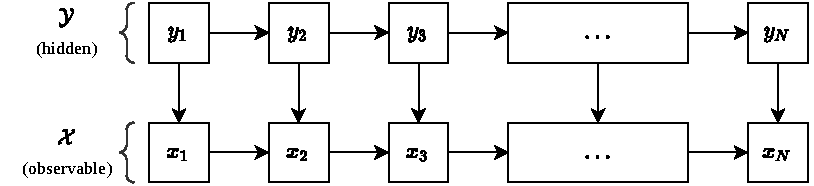
\includegraphics[width=0.90\textwidth]{hmm.pdf}
        \caption{In HMMs and CRFs, a hidden sequence $\mathcal{Y}$ is classified based on an an observable sequence $\mathcal{X}$.}
        \label{fig: HMM and CRF}
    \end{figure}

\subsection{Conditional Random Fields}
    \Glspl{crf} are a generalisation of HMM's that make fewer assumptions about probability distributions. Specifically, no assumptions on the dependencies among $x_{i} \in \mathcal{X}$ are made\cite{klinger2007classical}. Similar to how HMMs are Bayesian modelling applied to Markov processes, \glspl{crf} are an application of maximum entropy modelling to sequences\cite{klinger2007classical}.
\section{Word Embeddings \label{ssec: word embeddings}}

    \begin{figure}
        \centering
        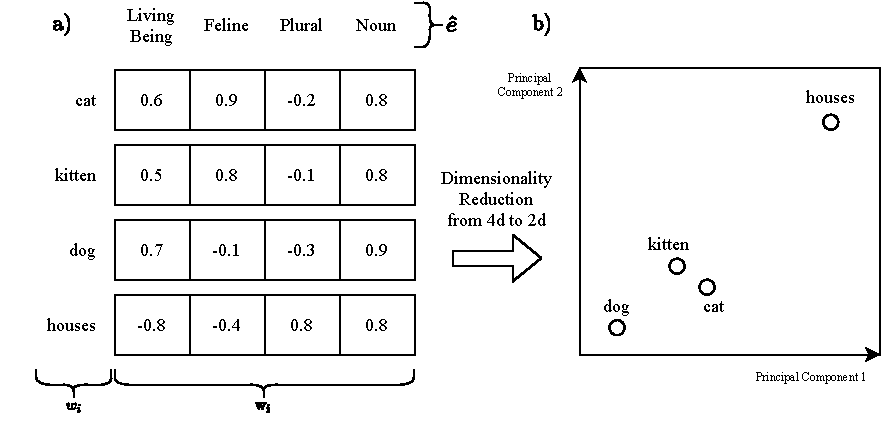
\includegraphics[width=0.9\textwidth]{embeddings.pdf}
        \caption{a) A schematic example of word \glspl{embedding} that represents each word in basis $\hat{e}$. In real-world embeddings, $\hat{e}$ is determined by the computer and has no human-understandable meaning. It also has much higher dimensionality. b) A graphical representation of the embedded words.}
        \label{fig:word embedding}
    \end{figure}

    For humans, (a large part of) learning a language is learning the mapping of words to their meanings such as ``dog" $\rightarrow$ pet with fur that makes ``woof" sound; ``table" $\rightarrow$ stable surface standing on legs etc. If a computer is to interpret textual information, we need to provide it with an analogous mapping. This is accomplished using word embeddings.
    Word \glspl{embedding} $\mathbf{w_i}$ are high-dimensional ($\approx 300$ dimensions) vectors of real numbers aiming to represent the semantic meaning of a word $w_i$. Fig. \ref{fig:word embedding} gives a simple example of such \glspl{embedding}. $\mathbf{w_i}$ are created by using large corpora of texts, (such as all Wikipedia articles, or a crawl through the entire internet) and using the context of words $w_i$ to learn their representation $\mathbf{w_i}$ in an unsupervised way. The basis for this is the assumption that similar words appear in similar contexts\cite{word2vec}.
    %Word \glspl{embedding} are at the heart of many \gls{nlp} applications and many pre-trained word \glspl{embedding} are available.
    The most prominent \glspl{embedding} are Google's, word2vec\cite{word2vec} and Stanford university's \gls{glove}\cite{glove} \glspl{embedding}. The lesser known \textit{ConceptNet Numberbatch} \glspl{embedding}\cite{conceptnet} build upon (and improve) both \gls{glove} and word2vec (see Sec. \ref{ssec: Numberbatch}).

    \subsection{GloVe \label{ssec: Glove}}
        \gls{glove}\cite{glove} (short for Global Vectors) is a mapping
        \[ \hat{f}(w_i) \rightarrow \mathbf{w_i}\]
        from words to \gls{embedding} vectors. It is trained on very large corpora such as Wikipedia or the entire internet. First, the co-occurence matrix $C_{ij}$ is created:

        \begin{equation}
        C_{ij} = \text{\# Co-occurences between words $i$ and $j$},
        \end{equation}

        where a co-occurence of two words means that they are featured within the same document, e.g. the same Wikipedia article or the same website. If there are $N_w$ words in the corpus, $C_{ij}$ is a $N_w \times N_w$ matrix, measuring the co-occurence between every word $w_i$ with every other word $w_j$.
        %For \gls{glove}, $N_w = \num{1.9e6}$ when trained on Wikipedia, $N_w = \num{2.2e6}$ when trained on a crawl of the entire internet.
        $C_{ij}$ is sparse, (meaning most entries are 0) as most words do not appear in the same context as most other words. By then performing dimensionality reduction (e.g. \gls{lda}) on $C_{ij}$, a dense representation of much lower dimensionality is obtained for every word. This representation is the word \gls{embedding}. For \gls{glove}, \glspl{embedding} are by default 300-dimensional\cite{glove}.

        Word2vec is trained in a similar way, though what counts as a co-occurence and how the dimensionality is reduced is slightly different\cite{word2vec}.

    \subsection{ConceptNet Numberbatch \label{ssec: Numberbatch}}

        ConceptNet is a open source semantic network that represents words (and short sequences of words commonly seen together) as nodes and the relationships between them as edges. An example is shown in Fig. \ref{fig: conceptnet}.
           \begin{figure}[h]
                \centering
                 \captionsetup{format=hang}
                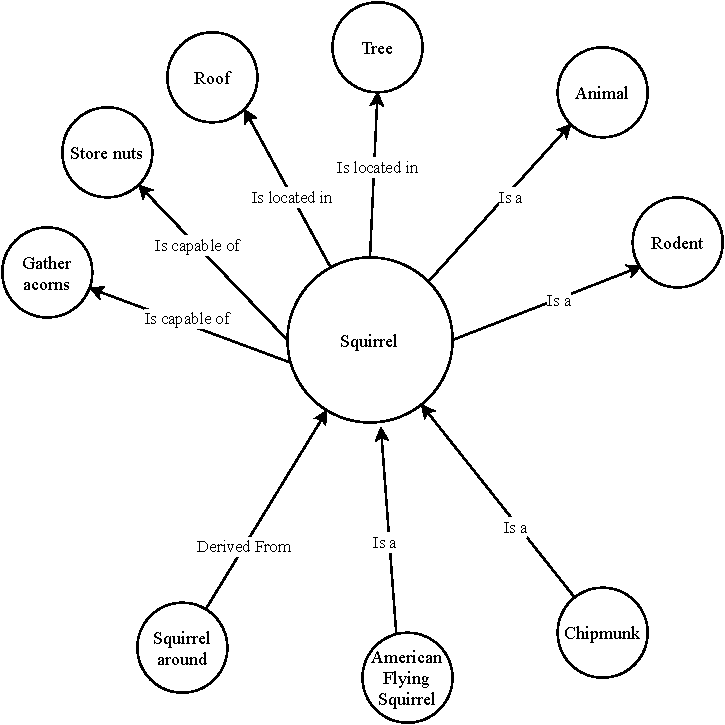
\includegraphics[width=0.7\textwidth]{conceptnet.pdf}
                \caption{Some of the connections of the word ``squirrel" in conceptNet. \label{fig: conceptnet}}
            \end{figure}

        By combining the ConceptNet network with other word \glspl{embedding} such as word2vec and \gls{glove} using a process called \textit{retrofitting}, a new, improved set of word \glspl{embedding}, the \textit{\gls{numberbatch}}, is created.

        \subsubsection{Retrofitting}
            Retrofitting uses a set of \glspl{embedding} $\mathbf{w_i}$, such as \gls{glove} or word2vec (Sec. \ref{ssec: Glove}) to infer new \glspl{embedding} $\Tilde{\mathbf{w_i}}$ that are both close to the original \glspl{embedding} and also close to their neighbours in the ConceptNet graph, by minimising the objective function
            \begin{equation}
                \Psi(W)=\sum_{i=1}^{N}\left[\alpha_{i}\left\|\mathbf{w}_{i}-\Tilde{\mathbf{w}}_{i}\right\|^{2}+\sum_{(i, j) \in E} \beta_{i j}\left\|\mathbf{w}_{i}-\mathbf{w}_{j}\right\|^{2}\right],
            \end{equation}
            where the sum is over all words included within the union of all words contained in ConceptNet with all words contained in the original \glspl{embedding}, $W$ is the set of all word \glspl{embedding} $\mathbf{w_i} \in W$, $E$ is the set of all edges within the ConceptNet graph, $\beta_{ij}$ is the weight of the edge between words $w_i$ and $w_j$ in the ConceptNet graph, and $\alpha_i$ are weights determining how important the previous \glspl{embedding} are compared to the edges within ConceptNet. How exactly $\alpha_i$ is determined is not explained within the original paper, but when a word is found within ConceptNet, that was not found within the \glspl{embedding}, $\alpha_i = 0$, allowing for a further expansion of the vocabulary.\cite{speer2017conceptnet}

        \subsubsection{Superior Performance}
            By combining word2vec, \gls{glove} and ConceptNet, the \gls{numberbatch} achieves superior performance in many word \gls{embedding} benchmarks\cite{speer2017conceptnet, conceptnetPerformance}.

        %\subsubsection{Mini Version}
            %As a convenience, the \gls{numberbatch} \glspl{embedding} are available as both more accurate 32-bit floating point numbers and as less accurate 8-bit integers. The 8-bit integer version allows for significantly smaller files (mini $\approx$ 50MB, full \glspl{embedding} $\approx$ 5GB) and loading times. We use the mini versions due to limited resources.

    \subsection{Similarity \label{ssec: cosine similarity}}
        The defining feature of word \glspl{embedding} is that semantically similar words have similar vectors. We can thus quantify the similarity $\eta_{ij}$ between two words $w_i, w_j$ as the cosine similarity of their \glspl{embedding}
        \begin{equation}
            \eta_{ij} = \text{cosine}(\mathbf{w_i}, \mathbf{w_j}) = \frac{\mathbf{w_i} \cdot \mathbf{w_j}}{|\mathbf{w_i}| |\mathbf{w_j}|}.
            \label{eq: cosine similarity}
        \end{equation}
        We use this notion of similarity heavily in this work.

    \subsection{Sentence Embeddings \label{ssec: utterance embeddings}}

    In the same way that words can be embedded based on a pre-trained set of \glspl{embedding}, sentences can be embedded also. Training the \glspl{embedding} doesn't work in the same way as for words (otherwise every sentence would have to be contained within the corpus for an \gls{embedding} to exist), but the concept is the same. A sentence is represented as a vector in a high-dimensional vector space. This allows a similarity between sentences to be computed as the cosine similarity (see Sec. \ref{ssec: cosine similarity}, Eq. \ref{eq: cosine similarity}). Examples include Google's universal sentence encoder\cite{GoogleEncoder} and Facebook's InferSent\cite{infersent}.

    \subsection{Limitations}
        \begin{figure}[h]
            \centering
            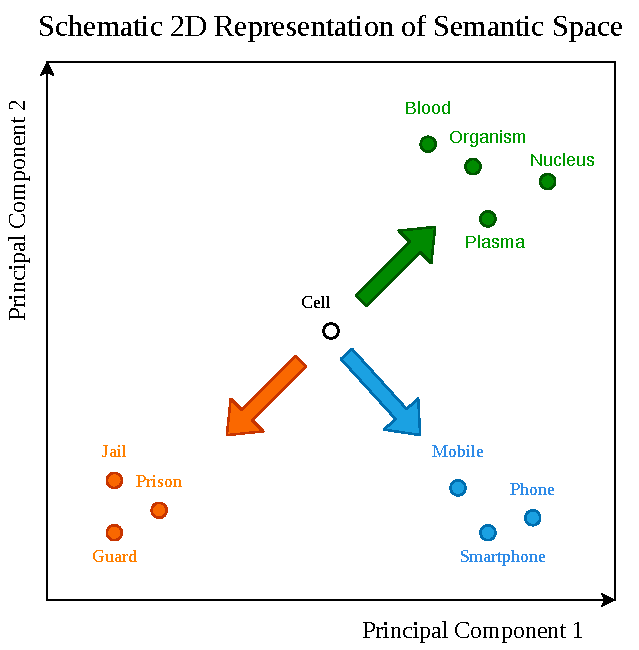
\includegraphics{ambiguous_embedding.pdf}
            \caption{Due to appearing frequently in contexts relating to biology, phones and prison, the word \gls{embedding} for the ambiguous word ``cell" is attracted to all three contexts in semantic space. The final \gls{embedding} lies somewhere in between the contexts and is a poor representation for all three meanings of ``cell".}
            \label{fig:ambiguous_embedding}
        \end{figure}

        Word \glspl{embedding} suffer from some limitations, the most significant of which is the problem of word-sense disambiguation, which occurs because words may have multiple meanings but only one \gls{embedding}. In the sentence
        \begin{align*}
            &\textit{``He went to the prison cell with his cell phone to extract blood cell samples}\\
            & \textit{from the inmates."}
        \end{align*}
        the word \textit{cell} appears 3 times and has a different meaning every time, but it has only one word \gls{embedding}. Because the method of \gls{embedding} is incapable of disambiguating the different meanings of the words, the word \gls{embedding} is poor: In the semantic vector space of word \glspl{embedding}, \textit{cell} will be attracted to words within its ``biology context", but also within its ``phone" context and within its ``prison" context, leading to a final \gls{embedding} somewhere in the middle, making it ineffective within all three contexts. The newest types of word \glspl{embedding}, such as BERT\cite{devlin2018bert} or ELMo\cite{peters2018elmo} address this problem by taking whole sentences as inputs and use the context of adjacent words to compute disambiguated word \glspl{embedding}.

\section{Conversation Analysis \label{sec: ca}}
\glsreset{ca}
The analysis of the structure of conversations falls within the field of \gls{ca}, a sub-field of linguistics. This section explores the key concepts from \gls{ca} that we use for our work. 
% CONVERSATION ANALYSIS FIRST
    \subsection{Utterances \label{ssec: utterances}}
        Within conversations, \glspl{utterance} are strings of words that begin and end with a clear pause. As an approximation, we are assuming that every \gls{utterance} corresponds to a sentence and in this thesis, sentences and \glspl{utterance} are considered synonyms.
        
        
    \subsection{Dialogue Acts \label{ssec: DAs}}
        The atomic unit within \gls{ca} is the \gls{da}. The \gls{da} describes the \textit{social action} of an \gls{utterance}. \Glspl{da} can be split into categories such as questions, greetings, statements of politeness, statements of agreement etc. for our work, we use the SWBD-DAMSL tag-set of 42 \glspl{da} featured in the \gls{swda} corpus (see Sec. \ref{ssec: swda})\cite{fang2012annotation, swda}. The most common \glspl{da} as well as their relative frequency within the \gls{swda} corpus is shown in table \ref{table: damsl das}.
        
        \begin{table}[ht]
        \begin{tabular}{|l|l|l|}
        \hline
            \textbf{SWBD-DAMSL}          & \textbf{Example}                                & \textbf{\%} \\ \hline
            Statement-non-opinion        & Me, I'm in the legal department.                & 36\%        \\ \hline
            Acknowledge (Backchannel)    & Uh-huh.                                         & 19\%        \\ \hline
            Statement-opinion            & I think it's great                              & 13\%        \\ \hline
            Agree/Accept                 & That's exactly it.                              & 5\%         \\ \hline
            Abandoned or Turn-Exit       & So, -                                           & 5\%         \\ \hline
            Appreciation                 & I can imagine.                                  & 2\%         \\ \hline
            Yes-No-Question              & Do you have to have any special training?       & 2\%         \\ \hline
            Non-verbal                   & {[}Laughter{]}, {[}Throat\_clearing{]}          & 2\%         \\ \hline
            Yes answers                  & Yes.                                            & 1\%         \\ \hline
            Conventional-closing         & Well, it's been nice talking to you.            & 1\%         \\ \hline
            Uninterpretable              & But, uh, yeah                                   & 1\%         \\ \hline
            Wh-Question                  & Well, how old are you?                          & 1\%         \\ \hline
            No answers                   & No.                                             & 1\%         \\ \hline
            Response Acknowledgement     & Oh, okay.                                       & 1\%         \\ \hline
            Hedge                        & I don't know if I'm making any sense or not.    & 1\%         \\ \hline
            Declarative Yes-No-Question  & So you can afford to get a house?               & 1\%         \\ \hline
            Other                        & Well give me a break, you know.                 & 1\%         \\ \hline
            Backchannel in question form & Is that right?                                  & 1\%         \\ \hline
            Quotation                    & You can't be pregnant and have cats             & .5\%        \\ \hline
            Summarize/reformulate        & Oh, you mean you went home.                     & .5\%        \\ \hline
            Affirmative non-yes answers  & It is.                                          & .4\%        \\ \hline
        \end{tabular}
        \caption{The most common SWBD-DAMSL dialogue acts, taken from \cite{swda}. The third column is the fractional frequency of the DA within the \gls{swda} corpus of short conversations (see Sec. \ref{ssec: swda}).}
        \label{table: damsl das}
        \end{table} 
        

    
    %\subsection{Adjacency Pairs \label{ssec: adjacency pairs}}
        
        %In a conversation, speech acts are part of a greater cohesive structure. In \gls{ca}, this is the structure of \textit{adjacency pairs}. Adjacency pairs are pairs of speech acts $(s_j, s_{j+1})$, in which the initial speech act with label $s_j$ is replied to by the response with label $s_{j+1}$. Examples include:
        %\begin{itemize}
        %    \item (question, answer)
        %    \item (greeting, greeting)
        %    \item (request, denial)
        %    \item (opinion, agreement) etc.
        %\end{itemize}
        %A conversation, on the \gls{utterance} level, is structured as a long string of such adjacency pairs.
        
    
    
\glsresetall
 % 3300 words
%{\let\clearpage\relax \chapter{Existing Work}}
\chapter{Existing Work}

% TODO: Change, no longer doing actual analysis
While to our knowledge no work exists that statistically analyses conversations on a large scale, the methods of analysis that we employ are common and well established. The first part of our analysis, in which we analyse a conversation as a string of many small \glspl{da} rests on \gls{da} classification and is addressed in Sec. \ref{ssec: da classification}. The second part of our analysis, which is concerned with analysing conversations as a trajectory through a semantic topic-space, uses topic modelling. Previous topic modelling work is explored in Sec. \ref{sec: topic analysis} -- \ref{ssec: topic labelling}.

\section{Dialogue Act Classification \label{ssec: da classification}}
    Dialogue acts (see Sec. \ref{ssec: DAs}) are often applied within the context of adjacency pairs (see \ref{ssec: adjacency pairs}). They have been used to analyse performance appraisal interviews\cite{ap_interview}, predict psychological disorders such as depression or social anxiety\cite{ap_psychological} or analyse politician's speech patterns\cite{ap_trump}.
    A lot of these are based on manually annotated transcriptions or are purely qualitative in nature. To automate DA annotation would make it significantly easier for researchers to process large data sets and quantify their findings. A model for classifying DAs could be written as 
    \begin{equation}
        \hat{f}_{da}: u_i \rightarrow l_i,
    \end{equation}
    where an utterance $u_i$ is mapped to a DA label $l_i$. Better models don't just map one utterance to one label, but consider the whole sequence of utterances $\mathcal{U}$ i.e.
    \begin{equation}
        \hat{f}_{da}: \mathcal{U} \rightarrow \mathcal{L}, \hspace{3em} u_i \in \mathcal{U}, \hspace{0.5em} l_i \in \mathcal{L} \hspace{0.5em} \forall \hspace{0.5em} i.
    \end{equation}
    
    DA classification is an active area of research and different neural network architectures are proposed to improve model performance. State of the art models for DA classification are summarised in \cite{DAgithub}. The comparison is shown in table \ref{table: da models}.
    
    \begin{table}[h]
    \centering
    \begin{tabular}{|l|l|l|}
    \hline
    \textbf{Model}                   & \textbf{Accuracy} & \textbf{Paper / Source}      \\ \hline
    SGNN                             & 83.1              & Ravi et al., 2018 \cite{ravi2018self}   \\ \hline
    CASA                             & 82.9              & Raheja et al., 2019\cite{raheja2019dialogue} \\ \hline
    DAH-CRF                          & 82.3              & Li et al., 2019 \cite{li2018dual}     \\ \hline
    ALDMN                            & 81.5              & Wan et al., 2018 \cite{wan2018improved}    \\ \hline
    CRF-ASN                          & 81.3              & Chen et al., 2018 \cite{chen2018dialogue}   \\ \hline
    Bi-LSTM-CRF                      & 79.2              & Kumar et al., 2017 \cite{kumar2017dialogue}  \\ \hline
    RNN with 3 utterances in context & 77.34             & Bothe et al., 2018 \cite{bothe2018context}  \\ \hline
    \end{tabular}
    \caption{State of the art models and their accuracies. Trained and evaluated on the SwDa corpus. There was only 84\% agreement among human annotators of the SwDa corpus, so the best models are almost as accurate as humans.\cite{swda}.}
    \label{table: da models}
    \end{table}
    
    \subsection{Bi-LSTM-CRF \label{sssec: kumar model}}
    For our work, we select the Bi-LSTM-CRF model\cite{kumar2017dialogue}, because of high model accuracy and because the authors released their source code. It combines a bidirectional recurrent network using LSTM neurons (see Sec. \ref{ssec: RNNs}) with a conditional random field (CRF) layer and word embeddings. Since we made changes to the model and re-implemented it, a more thorough explanation of the Bi-LSTM-CRF model along with a plot of the model (Fig. \ref{fig:kumar_model} can be found in the method section \ref{ssec: bi-lstm-crf} %TODO: Make CRF section

\section{Topic Extraction \label{sec: topic analysis}}

While \gls{da} classification is extensively and actively researched specifically within the context of conversations, topic extraction is not. Many techniques that work well in well-structured, regular text documents (such as newspaper articles or scientific papers) struggle within the context of conversations. These techniques, and the sparse attempts to apply them to conversations, are summarised in this section.

The usual approach to analysing topics in text is
\begin{enumerate}
    \item Segment the text into its different topics, i.e. determine where a topic changes (Sec. \ref{ssec: topic segmentation}).
    \item Label every segment with a topic, i.e. determine what a given segment is about (Sec. \ref{ssec: topic labelling}).
\end{enumerate}
Some methods, such as Purver et al.\cite{purver2006unsupervised}, do both at the same time.

Topic Extraction is used in a wide number of applications, for example in companies' live-chats, that automatically classify customer issues and send them to the most applicable support teams, or in content-sharing sites such as YouTube, that automatically generate tags for posts and videos to improve content recommendation\cite{queryClassification}. 
\section{Topic Segmentation \label{ssec: topic segmentation}}
Topic segmentation is a procedure that divides a text into sections, where each section significantly differs semantically from the previous. 
Consider the beginning of a conversation between podcast-host Joe Rogan and entrepreneur Elon Musk:\\

\BrText{$t_1$}{
    \begin{dialogue}
        
        \speak{Joe Rogan} Welcome back.
        
        \speak{Elon Musk}
        Here we go again.
        
        \speak{Joe Rogan}
        Great to see you and congratulations.
        \speak{Elon Musk}
        Thank you.
    \end{dialogue}
}

\vspace{1em} 
\hspace{2.5em} \myrulefill{20em}{\textsc{Topic Divider}}
\vspace{1em}
        
\BrText{$t_2$}{ 
    \begin{dialogue}
         
        
        \speak{Joe Rogan}
        You will never forget what is going on in the world when you think about when your child is born. You will know for the rest of this child’s life, you were born during a weird time.
        
        \speak{Elon Musk} [...]
    \end{dialogue}
}
\vspace{-0.3em}\\

\noindent A good topic segmentation algorithm splits this section of conversation at the indicated divider, where the topic changes from greetings to the birth of Elon Musk's child.


There are many approaches to topic segmentation that we explore. They are introduced in this section.

    %\subsection{Lexical Chain Segmentation} 
    %Lexical chain-based methods (such as LCSeg\cite{galley2003discourse}) try to identify semantically related sequences of words (lexical chains) based on term repetitions and then weights them according to frequency (chains containing more repeated terms receive a higher score) and chain length (shorter chains are more likely to be part of the same cohesive structure).\cite{galley2003discourse} \cite{hsueh2006automatic}. LCSeg is public and open for use.
    
    \subsection{Graph-based Segmentation} 
    Graph-based methods represent conversations as a fully connected weighted graph: nodes represent \glspl{utterance} $u_i$ and the weight of edges between nodes $u_i, u_j$ represent some measure of similarity $\eta_{ij}$ between $u_i, u_j$ (such as the cosine similarity between the two \gls{utterance} \glspl{embedding}, as is layed out in Sec. \ref{ssec: utterance embeddings}). Once the conversation is represented as a graph, a threshold weight $\eta_{\text{min}}$ between edges can be set, below which edges are removed. The remaining clusters of sentences defined by remaining edges give the segmentation of the conversation.\cite{malioutov2006minimum} A minimal example is shown in Fig. \ref{fig: graph seg}.
    
    \begin{figure}[ht]
    \centering
    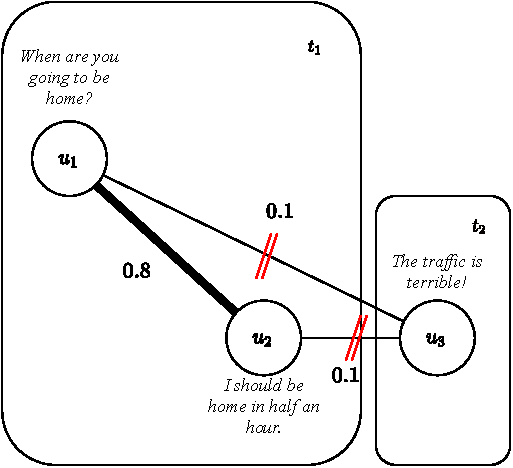
\includegraphics[width=0.7\textwidth]{graphSeg.pdf}
    \caption{Semantically different \glspl{utterance} have their connecting edge cut. The remaining clusters represent topics.\label{fig: graph seg}}
    \end{figure}
     
    \subsection{Bayesian Models}
    Some segmentation methods\cite{eisenstein2008bayesian, purver2006unsupervised, nguyen2012sits} combine segmentation with labelling using \gls{lda}. This is explored further in Sec. \ref{ssec: LDA}.
\section{Topic Labelling \label{ssec: topic labelling}}

Once a document has been segmented into semantically similar regions, for most tasks, they need to be labelled. There are two approaches to this:

\begin{enumerate}
    \item Supervised text classification, where every text is labelled with one (or multiple) topic-labels from a \textbf{predetermined set}\cite{surverTextClassification}. For example, one could label a newspaper article with a label from the set \{politics, sports, weather, finance \dots\}.
    \item Unsupervised topic modelling, where topic-labels are sets of words \textbf{contained within the document itself} and need to first be extracted.
\end{enumerate}

Text classification is often more accurate, but requires the user to impose a finite set of topics that a section can belong to. We explicitly want to avoid imposing a finite set of topics onto the conversations we analyse, so our analysis falls into the area of topic modelling. Common methods are explored here.


\subsection{Latent Dirichlet Allocation \label{ssec: LDA}}
    Latent Dirichlet allocation (LDA)\cite{blei2003latent} is the most common method for topic modelling. It was initially designed to model the topics of \textit{documents} within a \textit{corpus}, such as newspaper articles within an archive of newspapers. LDA is then capable of identifying words belonging to the same topic. The number of topics $k$ is a parameter of LDA and is set by the user.
    Within the context of conversations, the \textit{documents} are the conversation transcripts and the \textit{corpus} is the set of all transcripts.
    
    LDA is a \textit{generative model}, which makes the following assumptions about how a document is generated: There are $k$ topics that any word can be about e.g. $k=3$, where the topics are music, cooking and politics. Each of these topics is made up by the following words with an associated probability of appearing:
    \begin{align*}
        \textbf{Music:  }& \text{[(rock, 1\%), (pop, 0.8\%), (Mozart, 0.4\%), (mp3, 0.2\%), (Beatles, 0.2\%), \dots]}\\
        \textbf{Cooking:    }& \text{[(steak, 2.0\%), (dinner, 1.2\%), (knife, 1.0\%), (delicious, 0.6\%), \dots]}\\
        \textbf{Politics:   }& \text{[(Senate, 2.2\%), (MP, 1.8\%), (Trump, 0.9\%), (debating, 0.3\%), \dots]}.
    \end{align*} 
     
    Now, a document (such as a podcast transcript) is generated in the following way:
     
    \begin{enumerate}
        \item Choose a length of the document e.g. 1000 words.
        \item Choose a set of topics, as well as their probabilities of appearance within the document, e.g. \{(music, 80\%), (cooking, 20\%)\}
    \end{enumerate}
    
    For each word:
    \begin{enumerate}[leftmargin=6em]
    \setcounter{enumi}{2}
        \item A topic is randomly selected: with 80\% probability the topic is music with 20\% probability it is cooking.
        \item From within that topic (say music), a random word is selected with its given probability, e.g. 1\% of the time, the word ``rock" is chosen.
    \end{enumerate}
    
    The real model works \textbf{backwards} from these assumptions to compute the most likely parameters given the observed corpus.
    Mathemathically, LDA determines the parameters that are most likely to have generated the corpus by computing the probability of obtaining a given corpus $D$:
    
    \begin{equation}
        p(D \mid \alpha, \beta)=\prod_{d=1}^{M} \int p\left(T_{d} \mid \alpha\right)\left(\prod_{n=1}^{N_{d}} \sum_{z_{d n}} p\left(z_{d n} \mid T_{d}\right) p\left(w_{d n} \mid z_{d n}, \beta\right)\right) d T_{d},
    \end{equation}
    
    where $\alpha$ and $\beta$ are the parameters we would like to determine,
    the first product is over all $M$ documents $d$,
    the integral is over all possible sets (and probabilities) of topics $T_d$ included in $d$, 
    the second product is over all $N_d$ words that document $d$ contains, where $w_n$ is the $n^{th}$ word.
    The sum is over all topics $z_{dn}$, within $T_d$.
    The term after the sum can be recognised as the probability of drawing the word $w_{dn}$ after drawing the topic $z_{dn}$, which originates in the generative nature of the model.
    The term in the brackets is then the probability of drawing the entire document given that the random variable representing the set of topics is drawn to be $T_d$.
    
    Here, the parameter $\beta$ is a matrix containing the probabilities of every word to appear within every topic, and the parameter $\alpha$ is used as a parameter for drawing the set of topics $T_d$ from a Dirichlet distribution:
    
    \begin{equation}
        p(T \mid \alpha)=\frac{\Gamma\left(\sum_{i=1}^{k} \alpha_{i}\right)}{\prod_{i=1}^{k} \Gamma\left(\alpha_{i}\right)} T_{1}^{\alpha_{1}-1} \cdots T_{k}^{\alpha_{k}-1},
    \end{equation}
    where $k$ is the number of topics and the $d$ in the subscript of $T_d$ is replaced by the topic label for clarity. $\alpha$ is a $k$-dimensional vector with elements $> 0$ and $\Gamma(x)$ is the Gamma function.
    
    Once the LDA model is trained (i.e. a steady state of topic assignments exists), every word can be assigned a topic. By simple majority of topics within a segment, the segment can be labelled.
    
    \subsubsection{Limitations}
    LDA works very well when applied to similarly structured, similar length documents such as news articles\cite{blei2003latent, newman2006probabilistic} or scientific papers\cite{griffiths2004finding, wang2011collaborative}, but is known to struggle with documents that are too short, such as tweets and queries, or documents that contain many topics, such as books\cite{tang2014understanding}. Other weaknesses that are relevant to conversations include:
    
    \begin{itemize}
        \item The number $k$ of topics is fixed and must be subjectively imposed.
        \item Topics are uncorrelated as the Dirichlet topic distribution cannot capture correlations.
        \item Bag of word model: temporal evolution of topics can not be modelled as only word \textbf{counts} across the whole document are considered.
    \end{itemize}
    
    \subsubsection{LDA for Conversations \label{sssec: lda for conversations}}
    Conversations are irregular. They can contain many topics or are focused on just one, every topics can be described by many fitting words or by very few and conversation lengths vary significantly. In conjunction with mis-transcribed words that dilute topics, these issues mean that the generative LDA model, that assumes all documents are generated by the same ``recipe" does not perform well in this medium\cite{purver2006unsupervised, tang2014understanding}. A modified generative approach based on LDA is proposed independently by both Purver et al.\cite{purver2006unsupervised} and Eisenstein et al.\cite{eisenstein2008bayesian}, both of which specifically apply it to multi-party spoken discourse from recorded business meetings aggregated in the ICSI-MRDA corpus\cite{shriberg2004icsi}.
    
    \subsection{Keyphrase Extraction \label{ssec: keyphrase extraction}}
    Another, perhaps simpler, approach is to extract keyphrases (single or multi-word expressions that represent the main topics of a text) from the segmented sections in a process known as keyphrase extraction\cite{hasan2014automatic}. The extracted keyphrases (such as all nouns) represent the topic of the section.
    
    There are many keyphrase extraction methods, the one we evaluate is a graph-based model called TopicRank\cite{bougouin-etal-2013-topicrank}. Here, keyphrase candidates are extracted as noun phrases (phrases that grammatically act like nouns), such as:
    
    \begin{itemize}
        \item \textbf{The spotted puppy} is up for adoption.
        \item \textbf{The car wash} was out of order.
        \item She kindly offered water to \textbf{the gardener working in the hot sun.}
    \end{itemize}
    
    These phrases are identified using part of speech (POS) tagging.
        \subsubsection{Part of Speech Tagging \label{sssec: POS tagging}}
        
        Part of speech (POS) taggers are models 
        \begin{equation}
          \hat{f}_{\text{pos}}: \mathcal{S} \rightarrow \mathcal{P},
        \end{equation} 
        that label sequences of words $\mathcal{S}$(such as the words in a sentence) with their appropriate grammatical function $\mathcal{P}$, known as their part of speech tag. For example:
        
        \begin{equation*}
        \text{[The, house, is, green] $\rightarrow$ [article, noun, verb, adjective]}.
        \end{equation*}
        This tagging problem is approached almost exactly like the dialogue act tagging from Sec. \ref{ssec: da classification}.
        
        \subsubsection{Named Entity Recognition \label{sssec: NER}}
        Named entity recognition (NER) models
        \begin{equation}
          \hat{f}_{\text{ner}}: \mathcal{S} \rightarrow \mathcal{N},
        \end{equation} 
        extract words $\mathcal{N}$ in sequences of words $\mathcal{S}$ that describe a named entity such as a person, company or date and label them accordingly. For example:
        
        \begin{align*}
        \text{[Bill Gates, founded, Microsoft, in, 1975]} \rightarrow [& (\text{Bill Gates, person}), \\
                                                                       & (\text{Microsoft, company}), \\
                                                                       & (\text{1975, year})].
        \end{align*}
        This tagging problem is also approached almost exactly like the dialogue act tagging from Sec. \ref{ssec: da classification}.
        
        \subsubsection{Topic Clustering}
        
        Keyphrase-candidates are grouped into ``topics" if they share at least 25\% of words, excluding stop-words (which are words that don't add meaning, such as ``the").\cite{bougouin-etal-2013-topicrank}
        
        \subsubsection{Graph-Based Ranking}
        After keyphrase-candidates $c_i$ are extracted, the whole document is represented by a complete graph $G = (V, E)$, in which the vertices $V$ are topics $t_i$ and edges $E$ between two topics $t_i$ and $t_j$ are weighted according to the strength of their semantic relation. Here, two topics have a strong semantic relation if they appear close to each other in the document. Formally, the weights are defined to be
            \begin{align}
                w_{i, j} &=\sum_{c_{i} \in t_{i}} \sum_{c_{j} \in t_{j}} \operatorname{dist}\left(c_{i}, c_{j}\right) \\
                \operatorname{dist}\left(c_{i}, c_{j}\right) &=\sum_{p_{i} \in \operatorname{pos}\left(c_{i}\right)} \sum_{p_{j} \in \operatorname{pos}\left(c_{j}\right)} \frac{1}{\left|p_{i}-p_{j}\right|},
            \end{align}
        where pos$(c_i)$ represents all the offset positions (i.e. indices) of the candidate keyphrase $c_i$ within the document.
        
        The topics are then ranked according to the concept of ``voting": high-scoring topics contribute more to the score $S(t_j)$ of their connected topics $t_j$:
        
        \begin{equation}
            S\left(t_{i}\right)=(1-\lambda)+\lambda \times \sum_{t_{j} \in V_{i}} \frac{w_{j, i} \times S\left(t_{j}\right)}{\sum_{t_{k} \in V_{j}} w_{j, k}},
        \end{equation}
        where $V_i$ are the topics voting for $t_i$ and $\lambda$ is a damping factor.
        
        \subsubsection{Extracting the Topic-phrase}
        For each topic, only the most representative keyphrase candidate is selected as the phrase representing the topic. This topic-phrase is extracted for every topic $t_i$ by one of three different methods:
        \begin{enumerate}
            \item The keyphrase candidate that appears first in the document is the topic-phrase.
            \item The most frequent keyphrase candidate is the topic-phrase.
            \item The centroid of all candidates within $t_i$, which is defined to be the candidate most similar to all other candidates is the topic-phrase.\cite{bougouin-etal-2013-topicrank}
        \end{enumerate}
    
    The final topic labels are then defined by the topic-phrases above some minimum rank contained within the segment. This threshold allows the user to define a sensitivity for what constitutes a topic and what does not.
    
        \subsubsection{Limitations}
        Similarly to LDA, TopicRank performs very well when applied well-structured data such as journal papers, but is not evaluated for conversations.\cite{bougouin-etal-2013-topicrank}
     
    \section{Keyphrase Extraction \label{ssec: keyphrase extraction}}
    One labelling approach is the extraction of \glspl{keyphrase} (single or multi-word expressions that represent the main topics of a text) from the segmented sections\cite{hasan2014automatic}. The extracted \glspl{keyphrase} (such as all nouns) represent the topic of the section.
    
    There are many \gls{keyphrase} extraction methods, the one we evaluate is a graph-based model called TopicRank\cite{bougouin-etal-2013-topicrank}. Here, \gls{keyphrase} candidates are extracted as noun phrases (phrases that grammatically act like nouns), such as:
    
    \begin{itemize}
        \item \textbf{The spotted puppy} is up for adoption.
        \item \textbf{The car wash} was out of order.
        \item She kindly offered water to \textbf{the gardener working in the hot sun.}
    \end{itemize}
    
    These phrases are identified using part of speech tagging.
        \subsection{Part of Speech Tagging \label{sssec: POS tagging}}
        
        \Gls{pos} taggers are models 
        \begin{equation}
          \hat{f}_{\text{pos}}: \mathcal{S} \rightarrow \mathcal{P},
        \end{equation} 
        that label sequences of words $\mathcal{S}$(such as the words in a sentence) with their appropriate grammatical function $\mathcal{P}$, known as their part of speech tag. For example:
        
        \begin{equation*}
        \text{[The, house, is, green] $\rightarrow$ [article, noun, verb, adjective]}.
        \end{equation*}
        This tagging problem is approached almost exactly like the \gls{da} tagging from Sec. \ref{ssec: da classification}.
        
        
        \subsection{Topic Clustering}
        
        \Gls{keyphrase}-candidates are grouped into ``topics" if they share at least 25\% of words, excluding stop-words (which are words that don't add meaning, such as ``the").\cite{bougouin-etal-2013-topicrank}
        
        \subsection{Graph-Based Ranking}
        After \gls{keyphrase}-candidates $c_i$ are extracted, the whole document is represented by a complete graph $G = (V, E)$, in which the vertices $V$ are topics $t_i$ and edges $E$ between two topics $t_i$ and $t_j$ are weighted according to the strength of their semantic relation. Here, two topics have a strong semantic relation if they appear close to each other in the document. Formally, the weights are defined to be
            \begin{align}
                w_{i, j} &=\sum_{c_{i} \in t_{i}} \sum_{c_{j} \in t_{j}} \operatorname{dist}\left(c_{i}, c_{j}\right) \\
                \operatorname{dist}\left(c_{i}, c_{j}\right) &=\sum_{p_{i} \in \operatorname{pos}\left(c_{i}\right)} \sum_{p_{j} \in \operatorname{pos}\left(c_{j}\right)} \frac{1}{\left|p_{i}-p_{j}\right|},
            \end{align}
        where pos$(c_i)$ represents all the offset positions (i.e. indices) of the candidate \gls{keyphrase} $c_i$ within the document.
        
        The topics are then ranked according to the concept of ``voting": high-scoring topics contribute more to the score $S(t_j)$ of their connected topics $t_j$:
        
        \begin{equation}
            S\left(t_{i}\right)=(1-\lambda)+\lambda \sum_{t_{j} \in V_{i}} \frac{w_{j, i} S\left(t_{j}\right)}{\sum_{t_{k} \in V_{j}} w_{j, k}},
        \end{equation}
        where $V_i$ are the topics voting for $t_i$ and $\lambda$ is a damping factor.
        
        \subsection{Extracting the Topic-phrase}
        For each topic, only the most representative \gls{keyphrase} candidate is selected as the phrase representing the topic. This topic-phrase is extracted for every topic $t_i$ by one of three different methods:
        \begin{enumerate}
            \item The \gls{keyphrase} candidate that appears first in the document is the topic-phrase.
            \item The most frequent \gls{keyphrase} candidate is the topic-phrase.
            \item The centroid of all candidates within $t_i$, which is defined to be the candidate most similar to all other candidates is the topic-phrase.\cite{bougouin-etal-2013-topicrank}
        \end{enumerate}
    
    The final topic labels are then defined by the topic-phrases above some minimum rank contained within the segment. This threshold allows the user to define a sensitivity for what constitutes a topic and what does not.
    
        %\subsection{Limitations}
        %Similarly to \gls{lda}, TopicRank performs very well when applied to well-structured data such as journal papers, but is not evaluated for conversations.\cite{bougouin-etal-2013-topicrank}
\section{Latent Dirichlet Allocation \label{ssec: LDA}}
    \Gls{lda}\cite{blei2003latent} is the most common method for topic modelling. It was initially designed to model the topics of \textit{documents} within a \textit{corpus}, such as newspaper articles within an archive of newspapers. \gls{lda} is then capable of identifying words belonging to the same topic. The number of topics $k$ is a parameter of \gls{lda} and is set by the user.
    Within the context of conversations, the \textit{documents} are the conversation transcripts and the \textit{corpus} is the set of all transcripts.
    
    \gls{lda} is a \textit{generative model}, which makes the following assumptions about how a document is generated: There are $k$ topics that any word can be about e.g. $k=3$, where the topics are music, cooking and politics. Each of these topics is made up by the following words with an associated probability of appearing:
    \begin{align*}
        \textbf{Music:  }& \text{[(rock, 1\%), (pop, 0.8\%), (Mozart, 0.4\%), (mp3, 0.2\%), (Beatles, 0.2\%), \dots]}\\
        \textbf{Cooking:    }& \text{[(steak, 2.0\%), (dinner, 1.2\%), (knife, 1.0\%), (delicious, 0.6\%), \dots]}\\
        \textbf{Politics:   }& \text{[(Senate, 2.2\%), (MP, 1.8\%), (Trump, 0.9\%), (debating, 0.3\%), \dots]}.
    \end{align*} 
     
    Now, a document (such as a podcast transcript) is generated in the following way:
     
    \begin{enumerate}
        \item Choose a length of the document e.g. 1000 words.
        \item Choose a set of topics, as well as their probabilities of appearance within the document, e.g. \{(music, 80\%), (cooking, 20\%)\}
    \end{enumerate}
    
    For each word:
    \begin{enumerate}[leftmargin=6em]
    \setcounter{enumi}{2}
        \item A topic is randomly selected: with 80\% probability the topic is music with 20\% probability it is cooking.
        \item From within that topic (say music), a random word is selected with its given probability, e.g. 1\% of the time, the word ``rock" is chosen.
    \end{enumerate}
    
    The real model works \textbf{backwards} from these assumptions to compute the most likely parameters given the observed corpus.
    Mathematically, \gls{lda} determines the parameters that are most likely to have generated the corpus by computing the probability of obtaining a given corpus $D$:
    
    \begin{equation}
        p(D \mid \alpha, \beta)=\prod_{d=1}^{M} \int p\left(T_{d} \mid \alpha\right)\left(\prod_{n=1}^{N_{d}} \sum_{z_{d n}} p\left(z_{d n} \mid T_{d}\right) p\left(w_{d n} \mid z_{d n}, \beta\right)\right) d T_{d},
    \end{equation}
    
    where $\alpha$ and $\beta$ are the parameters we would like to determine,
    the first product is over all $M$ documents $d$,
    the integral is over all possible sets (and probabilities) of topics $T_d$ included in $d$, 
    the second product is over all $N_d$ words that document $d$ contains, where $w_n$ is the $n^{th}$ word.
    The sum is over all topics $z_{dn}$, within $T_d$.
    The term after the sum can be recognised as the probability of drawing the word $w_{dn}$ after drawing the topic $z_{dn}$, which originates in the generative nature of the model.
    The term in the brackets is then the probability of drawing the entire document given that the random variable representing the set of topics is drawn to be $T_d$.
    
    Here, the parameter $\beta$ is a matrix containing the probabilities of every word to appear within every topic, and the parameter $\alpha$ is used as a parameter for drawing the set of topics $T_d$ from a Dirichlet distribution:
    
    \begin{equation}
        p(T \mid \alpha)=\frac{\Gamma\left(\sum_{i=1}^{k} \alpha_{i}\right)}{\prod_{i=1}^{k} \Gamma\left(\alpha_{i}\right)} T_{1}^{\alpha_{1}-1} \cdots T_{k}^{\alpha_{k}-1},
    \end{equation}
    where $k$ is the number of topics and the $d$ in the subscript of $T_d$ is replaced by the topic label for clarity. $\alpha$ is a $k$-dimensional vector with elements $> 0$ and $\Gamma(x)$ is the Gamma function.
    
    Once the \gls{lda} model is trained (i.e. a steady state of topic assignments exists), every word can be assigned a topic.
    
    
    \subsection{LDA for Topic Labelling \label{ssec: lda for segmentation}}
    \gls{lda} is used for topic segmentation\cite{eisenstein2008bayesian, purver2006unsupervised, nguyen2012sits}, by checking how the topic distributions vary over time and placing a boundary between adjacent areas that show dissimilar distributions.
    By simple majority of topics within a segment, the segment can be labelled with the most-frequent words within that topic.
    
    \subsection{Limitations}
    \gls{lda} works very well when applied to similarly structured, similar length documents such as news articles\cite{blei2003latent, newman2006probabilistic} or scientific papers\cite{griffiths2004finding, wang2011collaborative}, but is known to struggle with documents that contain many topics, such as books\cite{tang2014understanding}. Other weaknesses that are relevant to conversations include:
    \begin{itemize}
        \item The number $k$ of topics is fixed and must be subjectively imposed.
        \item Topics are uncorrelated as the Dirichlet topic distribution cannot capture correlations.
        \item Bag of word model: temporal evolution of topics can not be modelled as only word \textbf{counts} across the whole document are considered.
    \end{itemize}
    
    \subsection{LDA for Conversations \label{sssec: lda for conversations}}
    Conversations are irregular. They can contain many topics or are focused on just one, every topics can be described by many fitting words or by very few and conversation lengths vary significantly. In conjunction with mis-transcribed words that dilute topics, these issues mean that the generative \gls{lda} model, that assumes all documents are generated by the same ``recipe" does not perform well in this medium\cite{purver2006unsupervised, tang2014understanding}. A modified generative approach based on \gls{lda} is proposed independently by both Purver et al.\cite{purver2006unsupervised} and Eisenstein et al.\cite{eisenstein2008bayesian}, both of which specifically apply it to multi-party spoken discourse from recorded business meetings aggregated in the ICSI-MRDA corpus \cite{shriberg2004icsi}. \newline
\glsresetall % 2000 words

{\let\clearpage\relax \chapter[Dialogue Act Classification]{Improving Dialogue Act Classification\label{cpt: Method Dialogue Acts}}}
%\chapter[Dialogue Act Classification]{Improving Dialogue Act Classification}
%We have three aims:
%\begin{enumerate}
%    \item Evaluate and improve existing automated dialogue act classification.
%    \item Evaluate and improve existing automated topic extraction method.
%    %\item Apply improved methods to a large number of conversations to determine the (statistical) ``bounds" of conversations.
%    \item Apply the improved methods to a large number of conversations to easily enable future work actually analysing said conversations.
%\end{enumerate}

\gls{da} classification is an active area of research, because it helps speech controlled devices (such as Google Home or Amazon Alexa) identify what the user wants\cite{daApplications}. As a reminder, in \gls{da} classification, we want to automatically map sentences to their embeddings, such as "Hello!" $\rightarrow$ question, "Do you live in London?" $\rightarrow$ Yes-or-No Question. We use the SWBD-DAMSL set of \glspl{da} introduced in \ref{table: damsl das}.

To improve \gls{da} classification, we select an existing hierarchical bi-directional \gls{lstm} \gls{model} Kumar et al. at IBM Research\cite{kumar2017dialogue} (for the reasons explained in Sec. \ref{sssec: kumar model}), re-implement it, modernise it and fix a bug. Our methods are described in this section.

%Sections ??? to ??? describes our methods and findings for the first aim, sections ??? to ??? for the second.

    %One way to view the structure of conversations is as a long string of adjacent \glspl{da}. Tagging these \glspl{da} automatically is an active area of research, because it helps speech controlled devices (such as Google Home or Amazon Alexa) identify what the user wants. All state of the art methods (see Sec. \ref{ssec: da classification}) use \glspl{rnn} for this task. 
    
    %\gls{da} classification is an active area of research, because it helps speech controlled devices (such as Google Home or Amazon Alexa) identify what the user wants\cite{daApplications}. We select an existing hierarchical bi-directional \gls{lstm} \gls{model} by Kumar et al.\cite{kumar2017dialogue} (for the reasons explained in Sec. \ref{sssec: kumar model}) and modernise it.
    
    \section{Training Data}
    To train \glspl{nn}, a set of training data of \glspl{utterance} $\mathcal{U}$ with their correctly labelled \glspl{da} $\mathcal{Y}$ is required. The two datasets that are commonly used in the literature are the \gls{swda} corpus (see Sec. \ref{ssec: swda}) and the Meeting Recorder Dialogue Dct (MRDa) corpus\cite{shriberg2004icsi}. We limit ourselves to the \gls{swda} corpus, because we believe the style of conversations in the \gls{swda} corpus to more closely resemble \textit{natural} conversations than the meeting transcriptions in the MRDA corpus.
    
    \section{Initial Model \label{method: kumar model}}
    The \gls{model} proposed in \cite{kumar2017dialogue} is a hierarchical Bi-LSTM-CRF \gls{model}, which first encodes \glspl{utterance} using an \gls{embedding} and \gls{lstm} layer and then uses these encoded \glspl{utterance} in a combination with another \gls{lstm} layer and a \gls{crf} layer to classify the Dialogue Act of every \gls{utterance}. The entire \gls{model} architecture is displayed in Fig. \ref{fig:kumar_model}.
    
    \begin{figure}[h]
        \centering
        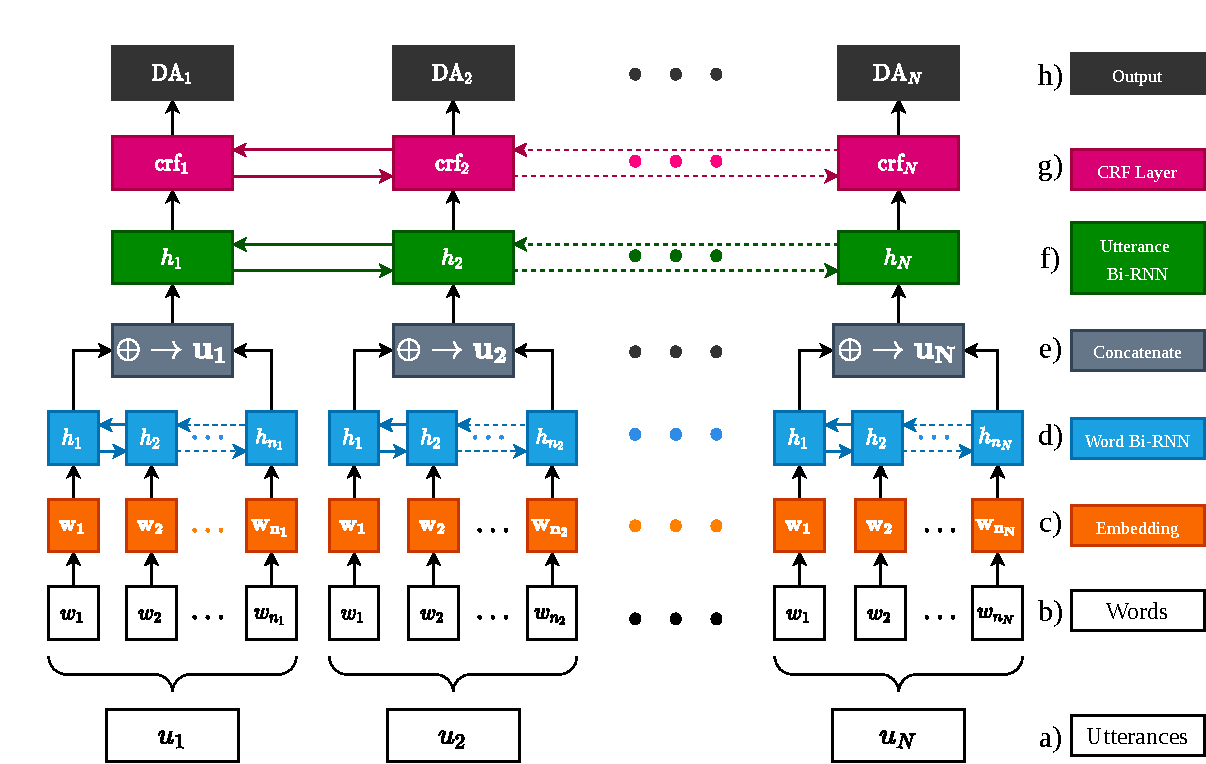
\includegraphics[width=\textwidth]{kumar.pdf}
        \caption{a) $N$ \glspl{utterance} $u_i$ are input into the \gls{model} as b) a list of words $w_1 \dots w_{n_i}$. In c), the words are individually embedded into vectors $\mathbf{w_j}$ (see Sec. \ref{ssec: word embeddings}). The first Bi-\gls{rnn} layer (on the word level), d), combines all $n_i$ words within $u_i$ into two vectors of numbers, one for the ``forward" direction and one for the ``backward" direction of the \gls{rnn} (see Sec. \ref{ssec: bidirectional RNN}). In e), these vectors are concatenated into one vector $\mathbf{u_i}$ that can be understood as the \gls{embedding} of the \gls{utterance} $u_i$. In f), these \gls{utterance} \glspl{embedding} are again combined using a bi-directional \gls{rnn} layer, but this time not just the two final states of the ``forward" and ``backward" direction are passed on, but all hidden states $h_i$ are (see Sec. \ref{ssec: outputting hidden states}). In g), a CRF layer (see Sec. \ref{fig: HMM and CRF}) makes the final classification, which is the sequence of \glspl{da} $\text{DA}_i$ associated with \glspl{utterance} $u_i$ shown in h).}
        \label{fig:kumar_model}
    \end{figure}
        
    \section{New Implementation}
        The code made public by the researchers is unfortunately not functional and as it is written in an outdated framework (tensorflow 1.3.0) for python, we were unable to fix the bugs. We therefore re-implement the \gls{model} in the more modern keras library CITE which is a high-level library that makes the low-level tensorflow 2.3.0 library more easily accessible. Our code is published on ??? (can not include name!).
        
    \section{Memory Problems}
        Due to limited resources, we ran the training and prediction process on a personal computer on a single NVIDIA GTX 1660Ti graphics card. This graphics card only has 6GB of internal memory, and because the \gls{model} needs to be able to handle conversations of up to 3000 sentences each up to 150 words of length, the storage used by the number of parameters of the \gls{model} far exceeds these 6GB ($\approx$25GB are required). We fix this issue by making the following assumption: The context of sentences matter, but only to an extent. It is unlikely that a \gls{da} of a sentence spoken 100 sentences ago, $DA_{i}$ ago impacts the \gls{da} classification of  $DA_{i + 100}$. Thus we split the text into chunks of 100 sentences, classify these chunks and re-assemble them.
    
        \subsubsection{Boundary Effects}
            The chunking process leads to unwanted boundary effects: at the boundary of each chunk, the \gls{model} loses the previous (or following) sentence's information. The context is lost. To mitigate this, we introduce a novel method of re-assembly of chunks. We don't only classify a chunk, say $u_{i}$ to $u_{i + 100}$, we also classify an offset chunk, say $u_{i + 50}$ to $u_{i + 150}$. We then re-assemble the classified chunks in a way that ensures that no \textbf{final} classification was made near a false boundary. The process is illustrated in Fig. \ref{fig:chunking process}. Given that we obtain the same accuracy as reported by Kumar et al. ($79.2 \pm 0.3\%$)\cite{kumar2017dialogue} using this method, it is clear that our assumption holds and this method does not significantly diminish the \gls{model}'s accuracy.
        
    \begin{figure}[h]
        \centering
        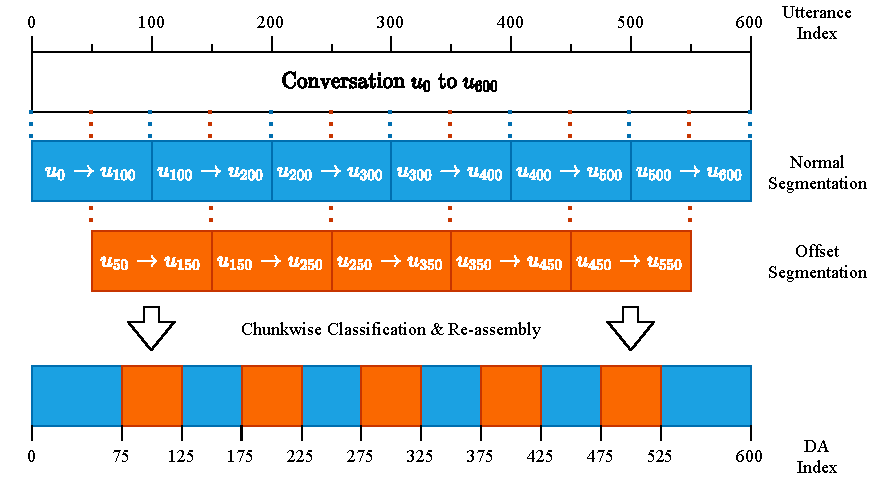
\includegraphics[width=\textwidth]{figures/chunks.pdf}
        \caption{The \glspl{utterance} are split into chunks of 100 twice: once starting at 0 (blue) and once offset, starting at 50 (orange). We classify each chunk independently and overlay them for the final classification so that each of the final \glspl{da} was classified as far from an artificial boundary as possible to minimise context information loss at boundaries.}
        \label{fig:chunking process}
    \end{figure}
        
    \section{Fixing Tokenisation Bug}
        After we re-implemented the \gls{model}, we achieve the accuracy of $79.2\% \pm 0.3\%$ that is reported by Kumar et al. However, we found a bug in the implementation which leads to some missed words and to some ends of sentences to be wrongly discarded: To embed an \gls{utterance}, it must first be split into its constituent words. Kumar et al. split the text on whitespace only, which leads to trailing punctation. For example, the sentence
        \begin{equation*}
            \text{Is that house's roof green?}
        \end{equation*}
        Gets split into the following tokens:
        \begin{equation*}
            \text{[Is, that, \color{red} house's, \color{black} roof, \color{red} green? \color{black}]}
        \end{equation*}
        The red tokens are not recognised as words within the pretrained \glspl{embedding} and their information is therefore lost. We fix this bug by splitting the same sentence in the following way:
        \begin{equation*}
            \text{[Is, that, house, ', s, roof, green, ?]}
        \end{equation*}
        The punctuation, as well as the single ``s" have its own \glspl{embedding} which leads to two improvements:
        \begin{enumerate}
            \item Words are no longer made invalid by the punctuation.
            \The information that the punctuation itself carries is now propagated to the \gls{model}.
        \end{enumerate}
        This change increases the \gls{model}'s accuracy to $81.0\% \pm 0.3\%$.
        

    
    \section{Changing Embeddings} 
    We change the \glspl{embedding} from \gls{glove} \glspl{embedding} used by Kumar et al.\cite{kumar2017dialogue} to the more sophisticated ConceptNet Numberbatch \glspl{embedding} (see Sec. \ref{fig: conceptnet}). We also allow the \gls{model} to change the \glspl{embedding} (via training) which optimises these general purpose \glspl{embedding} within this specific context of \gls{da} classification.
    
    \subsection{Modernising RNN cells}
    Kumar et al.\cite{kumar2017dialogue} use \gls{lstm} cells (see Sec. \ref{ssec: rnn architectures}) as the components of their \gls{rnn} layers. We instead use the more modern \gls{gru}\cite{chung2014empirical} neurons (see Sec. \ref{ssec: rnn architectures}), which require less time to train and are less prone to overfitting (an issue of machine learning models, in which the \gls{model} is too sensitive and understands random noise in the training data as a pattern leading to worse performance on unseen data)\cite{chung2014empirical}.
    
    \section{Evaluation \label{ssec: method my da model evaluation}}
    
    To evaluate our final \gls{model}, we randomly split the \gls{swda} data into 90\% training data and 10\% test data. The \gls{model} is trained only on the training data and only evaluated on the test data as is standard practice when evaluating any machine learning \gls{model} CITE. This process ensures that the \gls{model} has not seen the evaluation data (simulating the real application of the \gls{model}) leading to an unbiased accuracy measurement.
    Our final \gls{model}, which is the \gls{model} introduced by Kumar et al.\cite{kumar2017dialogue} with a fixed bug, using improved word \glspl{embedding}, and more modern \gls{rnn} components outperforms the original \gls{model} so significantly that it is currently the state of the art \gls{da} classification \gls{model}, achieving an accuracy of 
    \begin{equation}
        \text{accuracy} = 84.6 \% \pm 0.3\%,
        \label{eq: my da model accuracy}
    \end{equation}
    showing a greater accuracy than the (much more complex) previous state of the art \gls{model} by Ravi et al. at 83.1\%\cite{ravi2018self}. Perhaps more significantly, the humans that originally annotated the \gls{swda} corpus only had 84\% agreement\cite{swda}- meaning that this \gls{model} is as good as (if not slighly bettter than) individual humans at labelling \glspl{da}. \newline
\glsresetall % 1000 words
\chapter[Topic Extraction]{Improving Topic Extraction}
The second technique we intended to use for our analysis of conversations is that of topic extraction --- determining \textit{which} topics are addressed in a conversation and \textit{when}. In this chapter, we evaluate a number of usual topic modelling techniques within the context of conversations, determine key weaknesses and develop a novel topic extraction method that is more robust against these key weaknesses.

\section{Topic Segmentation Evaluation}
\subsection{A Lack of Corpora}
    Large corpora of training data for conversation topic segmentation do not exist, especially within the context of conversations, which causes two issues:
    \begin{enumerate}
        \item We can not train a \textbf{supervised} \gls{model} to detect boundary changes such as in \cite{joty2013topic}.
        \item Our quantitative evaluation is not representative of all conversations that we analyse and uncertainties are quite high.
    \end{enumerate}

\subsection{Our Evaluation Methods \label{method: segmentation evaluation}}
    In contexts other than conversations, algorithms are evaluated on chapters of medical textbooks\cite{eisenstein2008bayesian, simon2013leveraging}. Section titles are removed from the text and the algorithm is evaluated by how similarly its predicted boundaries are to the original section boundaries. Unfortunately, no such data exists for conversations.

    \subsubsection{Quantitative Evaluation}
        To quantify segmentation techniques, we annotate a 4 conversation sections (each ca. 250 sentences) by hand. To do this, we read through a transcript and place a boundary indicator in the text where we believe the topic of the conversation has changed. We try to annotate a representative sample of transcripts, but as this is a very time consuming process and conversation structure varies a lot, uncertainties are high and results statistically less significant than desired. We annotate sections from the podcasts shown in Table \ref{table: hand annotated podcasts}. They were chosen because we believe them to represent different types of conversations and a wide range of topics.

        \newcolumntype{b}{X}
        \newcolumntype{s}{>{\hsize=.5\hsize}X}

       \begin{table}[h]
       \centering
            \begin{tabularx}{0.9\textwidth}{| s | b | s | }
            \hline
            \textbf{Podcast Title}       & \textbf{Episode Title}                       & \textbf{Description}      \\ \hline
            Joe Rogan Experience         & \#1470 Elon Musk                             & Casual Conversation       \\ \hline
            Making Sense with Sam Harris & \#190 - How Should We Respond to Coronavirus & Expert Interview          \\ \hline
            143 Pixels                   & CaptLogun - World of Warcraft Classic        & Expert Conversation       \\ \hline
            6 Drunk 1 Sober              & Too Drunk                                    & Casual Group Conversation \\ \hline
            \end{tabularx}
            \caption{Podcasts of which we annotate a small subsection for evaluation purposes.}
            \label{table: hand annotated podcasts}
        \end{table}

    \subsubsection{Metric}
    We use the WindowDiff measure\cite{pevzner2002critique}, $w_d$ to rate segmentation. It moves a window of size $\Delta u$ across the segmented text and penalises the algorithm whenever the number of segmentation boundaries within the window does not match the ``true" (i.e. human annotated) number of boundaries for that window. Thus, a lower $w_d$ is better. We choose $\Delta u$ to be half the size of average segments in the true segmentation as is typical in the literature\cite{purver2006unsupervised}\cite{eisenstein2008bayesian}.

    \subsubsection{Future Improvements}
    For future research, we propose the creation of a data set similar to the medical textbook but for conversations, based on YouTube transcriptions:
    The video sharing platform YouTube allows video creators to split their video into segments called ``chapters"\cite{YoutubeChapters}. Some content creators, such as podcast host and artificial intelligence researcher Lex Fridman\cite{LexFridmanYoutube}, use these chapters to label topics. We hypothesise that if videos of conversations were transcribed and annotated with their ``chapter" titles, they could be used as a training set and evaluation set for topic segmentation in conversation.


%\subsection{Utterance Embedding Clustering \label{method: utterance embedding clustering}}
%    \begin{figure}[t]
%        \centering
%        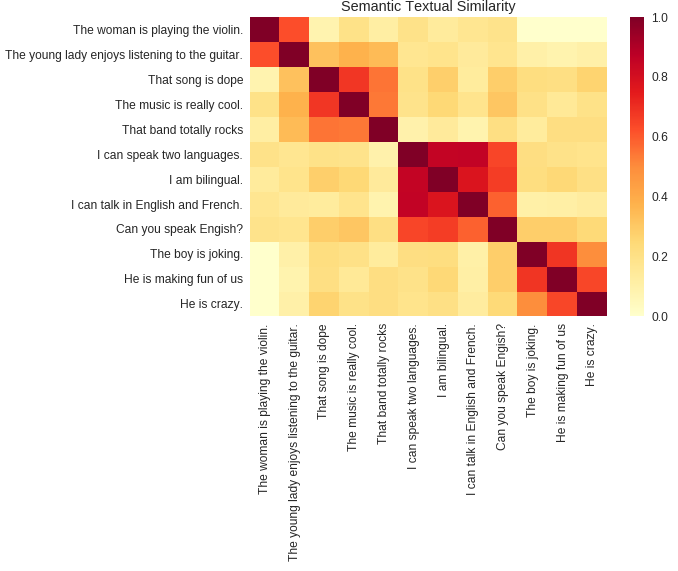
\includegraphics[width=0.8\textwidth]{sentence_similarity.png}
%        \caption{Using Google's universal sentence encoder, sentences are embedded and their similarity visualised. The colour of the field at (row, column) indicates the similarity between the sentence labels at (row, column). A darker colour indicates a stronger similarity.}
%        \label{fig:sentence similarity}
%    \end{figure}
%    Using \gls{utterance} embeddings, similar sentences can be clustered together, forming topics. A visual example showing sentence similarity is shown in Fig. \ref{fig:sentence similarity}.
%    Going through the transcript, once the cluster to which a sentence is assigned changes, a topic boundary is set. This theoretically allows for topic segmentation.
%
%    \subsubsection{Minimum Cut Graph Based \label{method: minimum cut}}
%
%        Firstly we evaluate the minimum cut based clustering method detailed in Sec. \ref{fig: graph seg} for conversations, in which all \glspl{utterance} above some threshold similarity are clustered. The key limitation within the context of conversation is that certain \glspl{utterance} appear within all topics. Consider the following sample of \glspl{utterance}:
%        \begin{table}[h]
%            \begin{tabular}{l|l}
%            $u_1$     & \textit{Rock music is the best!}                        \\
%            $u_2$     & \textit{Yeah man, rock is the best!}                    \\
%            \dots      &                                                         \\
%            $u_i$     & \textit{Lord of the Rings is the best movie ever made.} \\
%            $u_{i+1}$ & \textit{Yeah dude, Lord of the Rings really is the best.}              \\
%            \end{tabular}
%        \end{table}
%
%        Even though $u_1$ and $u_{i}$ correctly do not connect, $u_1$ connects to $u_2$, $u_{i}$ connects to $u_{i+1}$ and critically, $u_2$ connects to $u_{i+1}$. This last connection is made because the sentences are similar, in fact everything \textit{except for the topic} matches between these \glspl{utterance}. In conversation, sentences like $u_2$ and $u_{i+1}$ are abundant - leading to one giant connected component, which is a cluster that contains a large fraction of all nodes. We attempted to fine-tune the cutoff similarity, but either (almost) no sentences end up connected or all of them do.
%        From testing the method, we thus qualitatively identify two issues:
%        \begin{enumerate}
%            \item Sentences in conversation often carry little meaning, particularly those only acknowledge/agree with previous \glspl{utterance}. These acknowledgements act as bridges between clusters.
%            \item The minimum cut clustering method amplifies this because one \gls{utterance} acting as a bridge suffices to connect two clusters.
%        \end{enumerate}
%
%        The first issue is the key problem with using \gls{utterance} embeddings. While the minimum cut method is particularly vulnerable, other clustering methods also suffer from it.
%
%    \subsubsection{Other Clustering Methods}
%        Since the cutoff-based approach lead to issues, we try the following clustering methods in an attempt to minimize the vulnerability to falsely merged clusters:
%        \begin{itemize}
%            \item k-means clustering, in which the algorithm tries to separate samples in k groups of equal variance.
%            \item DBSCAN clustering, in which clusters are viewed as areas of high density separated by areas of low density.
%            \item Agglomerative clustering, in which a hierarchy of clusters is formed by assigning each \gls{utterance} its own cluster and then repeatedly merging the most similar clusters.
%        \end{itemize}
%        All three clustering methods were implemented using the python library scikit-learn\cite{scikit-learn}. These clustering methods qualitatively perform better than the minimum cut method, but each suffer from new issues. In k-means, imposing the number of topics $k$ is difficult as it varies heavily from conversation to conversation. In DBSCAN clustering, which requires neither a cutoff nor a number of topics, if data points are not inherently clustered (i.e. separated by areas of low density), the algorithm fails. This occured for a significant fraction of \glspl{utterance}. The most promising algorithm for clustering was the agglomerative clustering method, in which some topics could be clearly identified, but qualitative results were too poor to warrant further development and quantitative evaluation.
%
%    \subsubsection{Limitations}
%        No matter the clustering method, using sentence \glspl{embedding} is ineffective when analysing conversation topics. Some words in sentences don't contribute to the meaning act as unwanted bridges to other topics, but they can also \textit{dilute} the embedding. Consider the \glspl{utterance}
%
%
%        \begin{table}[h]
%            \begin{tabular}{l|l}
%            $u_1$     & \textit{Do you have any pets?}                    \\
%            $u_2$     & \textit{We had a light brown cat as a family pet when I was younger, but I don't now.}                        \\
%            \end{tabular}
%        \end{table}
%
%        Both \glspl{utterance} are about pets, but because the question and answer share almost no other words, and because the answer is very long, the sentences are deemed dissimilar by the \gls{model}. %TODO: actually get the sim value
%
%
%        % Put this as limitation in TopicRank
%        Another issue is that key-words are often not repeated but still understood as the topic. Consider the following \glspl{utterance}:
%
%        \begin{table}[h]
%            \begin{tabular}{l|l}
%            $u_1$     & \textit{Do you have any pets?}                    \\
%            $u_2$     & \textit{Yeah I've got a cat.}                        \\
%            \end{tabular}
%        \end{table}
%
%        The word ``pet" is not repeated  but from the context of the conversation it is clear that the topic is still ``pets".
%
%        The issue with the \gls{utterance} \gls{embedding} approach can be succinctly summarised as the following: \Glspl{Utterances} are more than just their topics. While the similarity of \glspl{utterances} is correlated with the similarity of the topics in which they lie, they are not equivalent. To make a more effective algorithm, the words representing topics must be first extracted.
%
%\subsection{Latent Dirichlet Allocation - BayesSeg \label{method: LDA}}
%    \begin{table}[]
%    \centering
%    \begin{tabular}{lllll}
%    \hline
%    \textbf{Topic 1}   & \textbf{Topic 2}    & \textbf{Topic 3}   & \textbf{Topic 4} & \textbf{Topic 5}  \\ \hline
%    technology   & models        & speakers     & wouldn't   & v\_a\_d     \\
%    u\_m\_t\_s   & reverberation & overlaps     & you'd      & worse       \\
%    routing      & voicing       & alignment    & agree      & t\_i-digits \\
%    transmission & multi-band    & region       & matter     & baseline    \\
%    i\_p         & targets       & breath       & depends    & I\_d\_a     \\
%    mobile       & phonemes      & laugh        & open       & percent     \\
%    packet       & effects       & native       & others     & italian     \\
%    university   & echo          & backchannels & feeling    & improvement \\
%    concerning   & combining     & laughing     & term       & adaptation  \\
%    networking   & insertions    & marks        & opposed    & latency     \\ \hline
%    \end{tabular}
%    \caption{Sample topics from recorded meeting dialogues, extracted by the modified \gls{lda} algorithm by Purver et al.\cite{purver2006unsupervised}. Words within topics are vaguely related, such as topic 1 concerning networking technology, or topic 3 about \glspl{da}. However, a lot of words don't fit well together and are unlikely to represent a topic.}
%    \label{table: modified lda topics}
%    \end{table}
%
%    One method of segmentation that attempts to extract topic-words is the modified \gls{lda} method \textit{BayesSeg} proposed by Eisenstein et al.\cite{eisenstein2008bayesian} (see Sec. \ref{ssec: topic segmentation}). We choose this method over the similar method presented by Purver et al.\cite{purver2006unsupervised}, because BayesSeg can be applied to individual documents, while the segmentation method by Purver et al. requires a whole corpus of documents. We only received access to the Spotify podcast corpus shortly before the date of submission of this thesis and so could not evaluate said method. However, from the examples shown in the original paper by Purver et al.\cite{purver2006unsupervised}, shown in Table \ref{table: modified lda topics}, we believe the algorithms suffer from similar limitations.
%
%    BayesSeg achieves the WindowDiff penalty score
%    \begin{equation}
%     w_d = 0.39 \pm 0.06
%    \end{equation}
%    when segmenting our annotated transcripts. The uncertainty is quite high because we had to annotate evaluation data manually, which is a time-consuming process and was thus limited to 4 transcripts. This is a significantly worse score than the value reported for the ICSI-MRDA corpus, $w_d = 0.312$\cite{eisenstein2008bayesian}.
%
%    While the results could agree due to the high uncertainty, we hypothesise the following reason for this reduction in performance instead: \gls{lda} assumes that every word is generated by sampling a topic, which is a distribution over words. Every word is assumed to be part of a topic. In more robust media, such as scientific papers or newspaper articles, this may be an appropriate approximation: if the aim is to convey information efficiently, most words will be related to the topic that is discussed. To an extent, the formal business meetings in the ICSI-MRDA corpus still fit this description. In more casual conversations, however, a lot of words are not related to the topic discussed: they act as statements of politeness, as acknowledgements, to fill breaks of awkward silence or to be entertaining\cite{searle1965speech}. This could be an explanation for the worse performance of BayesSeg in casual conversations, and could be further investigated in future work by evaluating performance on more and less formal conversations.
%
%      We identify two further key issues with \gls{lda}-based methods for casual conversation and use examples from the segmentation \gls{model} by Purver et al., shown in Table \ref{table: modified lda topics}, to support them:
%    \begin{enumerate}
%        \item The lack of correlations captured by \gls{lda} as well as its inability to \gls{model} temporal topic evolution means that unrelated topics can be falsely grouped together. For example ``university" does not fit in Topic 1, and ``Italy" does not fit in Topic 5.
%        \item The generative assumption that every word describes a topic leads to topics of words that do not have coherent semantic meaning and appear frequently, reducing the effectiveness of segmentation. An example is Topic 4.
%    \end{enumerate}
%
%
%    %TODO: lda cant do correlations, if two different topics appear together, it sticks them together (t2, t3, t5 (italian)).
%    %Also: forcing every word to belong to topic leads to misfits e.g. "combining" in 2, "concerning" in 1,
%
%\subsection{TopicRank \label{method: topic rank}}
%
%Utterance embedding based methods (Sec. \ref{method: utterance embedding clustering}) as well as \gls{lda}-based methods (Sec. \ref{method: LDA} are somewhat ineffective for the segmentation of conversation in part because they assume that every word in every \gls{utterance} contributes to the topic of the conversation, which is false.
%TopicRank\cite{bougouin-etal-2013-topicrank} (see Sec. \ref{ssec: keyphrase extraction}) offers a promising alternative approach: it first extracts \glspl{keyphrase} that are likely to represent topics and discards the rest.
%
%\subsubsection{Evaluation}
%We use TopicRank on our hand-annotated transcripts and compare its selected topic-phrases against human-annotated topic-phrases. If a topic-phrase extracted by TopicRank, $t_{\text{TR}}$ has a similarity greater than

\section[Clustering]{Utterance Embedding Clustering \label{method: utterance embedding clustering}}
    \begin{figure}[t]
        \centering
        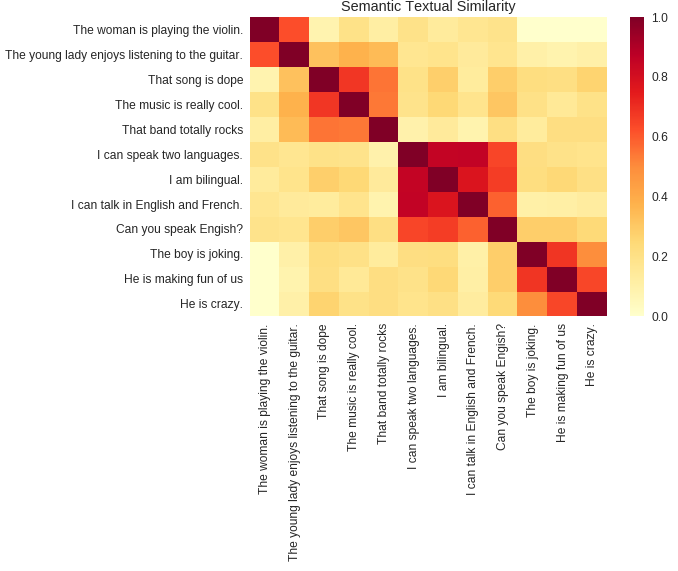
\includegraphics[width=0.8\textwidth]{sentence_similarity.png}
        \caption{Using Google's universal sentence encoder, sentences are embedded and their similarity visualised. The colour of the field at (row, column) indicates the similarity between the sentence labels at (row, column). A darker colour indicates a stronger similarity.}
        \label{fig:sentence similarity}
    \end{figure}
    As a first topic segmentation approach, we follow the graph-based technique introduced by Malioutov et al.\cite{malioutov2006minimum} (see Sec. \ref{ssec: topic segmentation}). Using \gls{utterance} \glspl{embedding} to cluster semantically similar sentences, forming topics. Going through the transcript, once the cluster to which a sentence is assigned changes, a topic boundary is set. This theoretically allows for topic segmentation. A visual example showing clusters of similar sentences is shown in Fig. \ref{fig:sentence similarity}.

    \subsection{Minimum Cut Graph Based \label{method: minimum cut}}

        Firstly we evaluate the minimum cut based clustering method detailed in Sec. \ref{fig: graph seg} for conversations, in which all \glspl{utterance} above some threshold similarity are clustered.
        
        Unfortunately, this approach does not work well: The key limitation within the context of conversation is that certain \glspl{utterance} appear within all topics. Consider the following sample of \glspl{utterance}:
        \begin{table}[h]
            \begin{tabular}{l|l}
            $u_1$     & \textit{Rock music is the best!}                        \\
            $u_2$     & \textit{Yeah man, rock is the best!}                    \\
            \dots      &                                                         \\
            $u_i$     & \textit{Lord of the Rings is the best movie ever made.} \\
            $u_{i+1}$ & \textit{Yeah dude, Lord of the Rings really is the best.}              \\
            \end{tabular}
        \end{table}

        \Glspl{utterance} $u_1$ and $u_2$ connect, $u_{i}$ connects to $u_{i+1}$ and even though $u_1$ and $u_{i}$ correctly do not connect, $u_2$ mistakenly connects to $u_{i+1}$. \color{red} \textbf{TODO: get values}. \color{black} This last connection is made because the sentences are similar, in fact everything \textit{except for the topic} matches between these \glspl{utterance}. In conversation, sentences like $u_2$ and $u_{i+1}$ are abundant --- leading to one giant connected component (a cluster that contains a large fraction of all nodes). We attempted to fine-tune the cutoff similarity, but either (almost) no sentences end up connected or all of them do.


    \subsection{Other Clustering Methods}
        Since the cutoff-based approach lead to issues, we try the following clustering methods in an attempt to minimise the vulnerability to falsely merged clusters:
        \begin{itemize}
            \item k-means clustering, in which the algorithm tries to separate samples in k groups of equal variance.
            \item DBSCAN clustering, in which clusters are viewed as areas of high density separated by areas of low density.
            \item Agglomerative clustering, in which a hierarchy of clusters is formed by assigning each \gls{utterance} its own cluster and then repeatedly merging the most similar clusters.
        \end{itemize}
        All three clustering methods were implemented using the python library scikit-learn\cite{scikit-learn}. While some clustering methods (especially agglomerative clustering) qualitatively perform better than the minimum cut method, none work well enough to warrant time-consuming quantitative evaluation.

        %These clustering methods qualitatively perform better than the minimum cut method, but each suffer from new issues. In k-means, imposing the number of topics $k$ is difficult as it varies heavily from conversation to conversation. In DBSCAN clustering, which requires neither a cutoff nor a number of topics, if data points are not inherently clustered (i.e. separated by areas of low density), the algorithm fails. This occured for a significant fraction of \glspl{utterance}. The most promising algorithm for clustering was the agglomerative clustering method, in which some topics could be clearly identified, but qualitative results were still too poor to warrant further development and quantitative evaluation.

    \subsection{Limitations}
        No matter the clustering method, using sentence \glspl{embedding} is ineffective when analysing conversation topics. \Glspl{utterance} in casual conversations are more than just their topics, many words dilute the semantics of an \gls{utterance} to such an extent that it becomes
        \begin{enumerate}
            \item indistinguishable from other \glspl{utterance} talking about different topics
            \item too dissimilar to other \glspl{utterance} talking about the same topic
        \end{enumerate}
        making it a poor method for topic segmentation.


        %A lot of words Some words in sentences don't contribute to the meaning act as unwanted bridges to other topics, but they can also \textit{dilute} the embedding. Consider the \glspl{utterance}


        %\begin{table}[h]
        %    \begin{tabular}{l|l}
        %    $u_1$     & \textit{Do you have any pets?}                    \\
        %    $u_2$     & \textit{Yeah, well, we had a light brown cat when I was younger, but I don't now.}                        \\
        %    \end{tabular}
        %\end{table}

        %Both \glspl{utterance} are about pets, but because the question and answer share almost no other words, and because the answer is very long, the sentences are deemed dissimilar by the model. %TODO: actually get the sim value



        %The issue with the \gls{utterance} \gls{embedding} approach can be succinctly summarised as the following: \Glspl{utterance} are more than just their topics. While the similarity of \glspl{utterance} is correlated with the similarity of the topics in which they lie, they are not equivalent. To make a more effective algorithm, the words representing topics must be first extracted.

\section[LDA BayesSeg]{Latent Dirichlet Allocation - BayesSeg \label{method: LDA}} 
    \begin{table}[]
    \centering
    \begin{tabular}{lllll}
    \hline
    \textbf{Topic 1}   & \textbf{Topic 2}    & \textbf{Topic 3}   & \textbf{Topic 4} & \textbf{Topic 5}  \\ \hline
    technology   & models        & speakers     & wouldn't   & v\_a\_d     \\
    u\_m\_t\_s   & reverberation & overlaps     & you'd      & worse       \\
    routing      & voicing       & alignment    & agree      & t\_i-digits \\
    transmission & multi-band    & region       & matter     & baseline    \\
    i\_p         & targets       & breath       & depends    & I\_d\_a     \\
    mobile       & phonemes      & laugh        & open       & percent     \\
    packet       & effects       & native       & others     & italian     \\
    university   & echo          & backchannels & feeling    & improvement \\
    concerning   & combining     & laughing     & term       & adaptation  \\
    networking   & insertions    & marks        & opposed    & latency     \\ \hline
    \end{tabular}
    \caption{Sample topics from recorded meeting dialogues, extracted by the modified LDA algorithm by Purver et al.\cite{purver2006unsupervised}. Words within topics are vaguely related, such as topic 1 concerning networking technology, or topic 3 about conversations. However, a lot of words don't fit well together and are unlikely to represent a topic.}
    \label{table: modified lda topics}
    \end{table}
    
    One method of segmentation that attempts to extract topic-words is the modified LDA method \textit{BayesSeg} proposed by Eisenstein et al.\cite{eisenstein2008bayesian} (see Sec. \ref{ssec: topic segmentation}). We choose this method over the similar method presented by Purver et al.\cite{purver2006unsupervised}, because BayesSeg can be applied to individual documents, while the segmentation method by Purver et al. requires a whole corpus of documents. We only received access to the Spotify podcast corpus shortly before the date of submission of this thesis and so could not evaluate said method. However, from the examples shown in the original paper by Purver et al.\cite{purver2006unsupervised}, shown in Table \ref{table: modified lda topics}, we believe the algorithms suffer from similar limitations.
    
    BayesSeg achieves the WindowDiff penalty score
    \begin{equation}
     w_d = 0.39 \pm 0.06
    \end{equation} 
    when segmenting our annotated transcripts. The uncertainty is quite high because we had to annotate evaluation data manually, which is a time-consuming process and was thus limited to 4 transcripts. This is a significantly worse score than the value reported for the ICSI-MRDA corpus, $w_d = 0.312$\cite{eisenstein2008bayesian}.
    
    We hypothesis that the reduction in performance comes from the change in media: we believe podcast conversations to be more casual, less topic-oriented (less expert knowledge) and less structured than dialogue in meetings, leading to a more difficult segmentation.
    
    %While the results could agree due to the high uncertainty, we hypothesise the following reason for this reduction in performance instead: LDA assumes that every word is generated by sampling a topic, which is a distribution over words. Every word is assumed to be part of a topic.
    %In more robust media, such as scientific papers or newspaper articles, this may be an appropriate approximation: if the aim is to convey information efficiently, most words will be related to the topic that is discussed.
    %To an extent, the formal business meetings in the ICSI-MRDA corpus still fit this description, sentences in meetings are trying to convey information efficiently, they largely relate to the topic at hand. In more casual conversations, however, a lot of words are not related to the topic discussed: they act as statements of politeness, as acknowledgements, to fill breaks of awkward silence or to be entertaining\cite{searle1965speech}.
    %This could be an explanation for the worse performance of BayesSeg in casual conversations, and could be further investigated in future work by evaluating performance on more and less formal conversations.
    
      We identify two further key issues with LDA-based methods for casual conversation and use examples from the segmentation model by Purver et al., shown in Table \ref{table: modified lda topics}, to support them:
    \begin{enumerate}
        \item The lack of correlations captured by LDA as well as its inability to model temporal topic evolution means that unrelated topics can be falsely grouped together. For example ``university" does not fit in Topic 1, and ``Italy" does not fit in Topic 5.
        \item The generative assumption that every word describes a topic leads to topics of words that do not have coherent semantic meaning and appear frequently, reducing the effectiveness of segmentation. An example is Topic 4.
    \end{enumerate}
    
    
    %TODO: lda cant do correlations, if two different topics appear together, it sticks them together (t2, t3, t5 (italian)). 
    %Also: forcing every word to belong to topic leads to misfits e.g. "combining" in 2, "concerning" in 1, 
\section{TopicRank \label{method: topic rank}}

Utterance \gls{embedding} based methods (Sec. \ref{method: utterance embedding clustering}) as well as \gls{lda}-based methods (Sec. \ref{method: LDA} are somewhat ineffective for the segmentation of conversation in part because they assume that every word in every \gls{utterance} contributes to the topic of the conversation, which is false.
TopicRank\cite{bougouin-etal-2013-topicrank} (see Sec. \ref{ssec: keyphrase extraction}) offers a promising alternative approach: it first extracts \glspl{keyphrase} that are likely to represent topics and discards the rest.

\subsection{Evaluation}
\begin{figure}
    \centering
    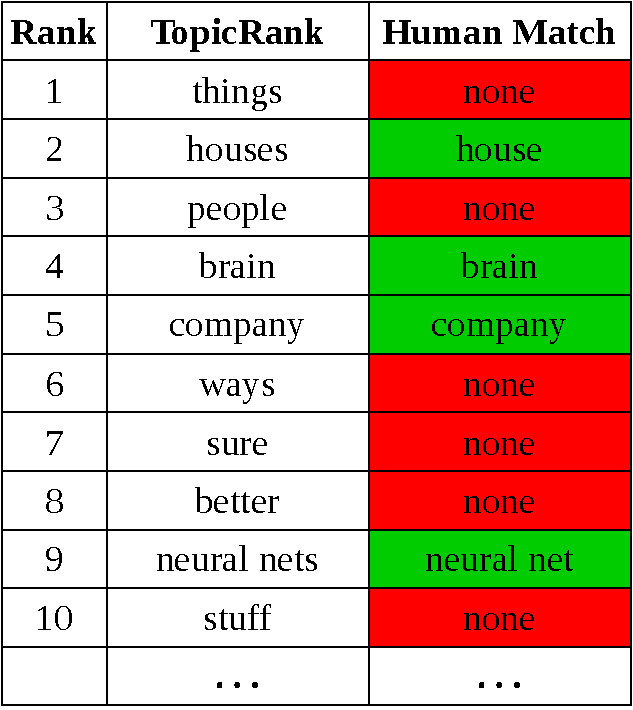
\includegraphics[width=0.5\textwidth]{topicRankEval.pdf}
    \caption{Top 10 \glspl{keyphrase} as determined by TopicRank and human matches where appropriate.}
    \label{fig: topicrank eval}
\end{figure}
We use TopicRank on our hand-annotated transcripts and compare its selected topic-phrases against human-annotated topic-phrases. If a given transcript has $N_{h}$ human annotated \glspl{keyphrase}, the top $N_{h}$ \glspl{keyphrase} as determined by the TopicRank algorithm are extracted. If a \gls{keyphrase} extracted by TopicRank or its plural/singular version is also found to be a \gls{keyphrase} by the human annotator, it is a match. On the 4 annotated transcripts, TopicRank achieves an accuracy (i.e. overlap with human \glspl{keyphrase})
\begin{equation}
    \text{accuracy} = 0.45 \pm 0.20.
    \label{eq: topic rank accuracy}
\end{equation}

\subsection{Limitations}
Fig. \ref{fig: topicrank eval} shows the top 10 highest ranked \glspl{keyphrase} and its human annotated counterpart if it exists. This illustrates two limitations of TopicRank:
\begin{enumerate}
    \item Abstract nouns such as ``things", ``people" or ``ways" are identified as topics even though they do not indicate a topic.
    \item Adjectives that are included as \gls{keyphrase} candidates, such as ``better" most often do not indicate a topic.
\end{enumerate}

% Put this as limitation in TopicRank
Another issue is that key-words are often not repeated but still understood as the topic. Consider the following \glspl{utterance}:

\begin{table}[h]
    \begin{tabular}{l|l}
    $u_1$     & \textit{Do you have any pets?}                    \\
    $u_2$     & \textit{Yeah I've got a cat.}                        \\
    \end{tabular}
\end{table}

The word ``pet" is not repeated  but from the context of the conversation it is clear that the topic is still ``pets". To improve the topic matching, we thus need to match semantically \textbf{similar} words instead of just matching equal words.

\section{GEEK Algorithm}

    \begin{figure}
        \centering
        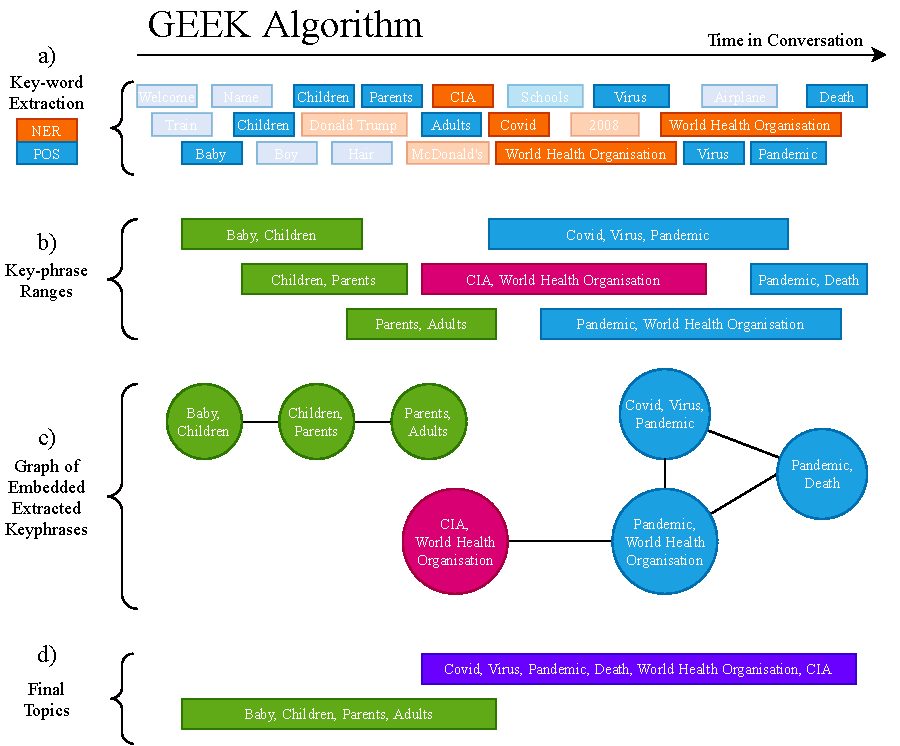
\includegraphics[width=\textwidth]{geek.pdf}
        \caption{A toy example showing how GEEK works.\newline a) \Glspl{keyphrase} are extracted as nouns and proper nouns using \gls{pos} tagging (blue) and as named entities using \gls{ner} (orange). The words on a transparent background are discarded because they are not similar to other nearby \glspl{keyphrase}.\newline b) The \glspl{keyphrase} are matched with similar nearby \glspl{keyphrase} and the range of their effect is determined. \newline c) A graph of \glspl{keyphrase} is created based on \gls{keyphrase}-range overlap and similarity. The colour is meant to serve as a visualisation of embeddings (similar colour $\rightarrow$ similar embedding).\newline
        d) The topics are the \glspl{keyphrase} in connected components in the graph. They range from the earliest \gls{keyphrase} occurence to the latest. The meaning of the final topic is influenced by all connected \glspl{keyphrase} (shown here as colour mixing).
        }
        \label{fig:geek architecture}
    \end{figure}

We use the TopicRank approach and build upon it to develop an algorithm that both segments and labels topics. We call this improved algorithm the \gls{geek} algorithm. \gls{geek} extracts \glspl{keyphrase}, but uses different criteria to make a different selection than TopicRank.
It then uses \gls{embedding}-based similarity to determine cohesive sections of the transcript. An example of how \gls{geek} works is shown in Fig. \ref{fig:geek architecture}.

\gls{geek} is based on the following assumptions:

\begin{enumerate}
    \item Topics are described by a small number of \glspl{keyphrase}. We assume \glspl{keyphrase} to exclusively be nouns, proper nouns and named entities, such as \textit{family}, \textit{music}, \textit{Donald Trump, the CIA} or \textit{Tesla}.
    \item Topics are sections within the text that feature similar \glspl{keyphrase}. \glspl{keyphrase} that are only mentioned once can not represent a topic.
    \item There can be more than one active topic: topics can overlap and smaller sub-topics can be discussed within larger topics.
    \item If the gap between related \glspl{keyphrase} is too large, they do not belong to the same segment.
\end{enumerate}
    
    \vbox{ %don't pagebreak this.
        \subsection{Hyperparameters}
        The hyperparameters that the user needs to set to use \gls{geek} are as follows:
        
        \newcolumntype{t}{>{\hsize=.15\hsize}X}
        \newcolumntype{L}{>{\hsize=.7\hsize}X}
        \begin{table}[H]
            \centering
            \begin{tabularx}{0.9\textwidth}{| t | L | t |}
            \hline
            \textbf{Symbol} & \textbf{Description} & \textbf{Chosen Value} \\ \hline
            $\Delta_{\text{max}}$     & The maximum gap between matching \glspl{keyphrase} for them to be considered in the same segment & 11                    \\ \hline
            $\eta_{\text{min}}$     & The minimum cosine similarity of two word \glspl{embedding} for their words to be considered similar. & 0.55                        \\ \hline
            $T_{\text{min}}$ & Minimum number of \glspl{utterance} a topic must span. & 3 \\ \hline
    
            \end{tabularx}
        \end{table}
    }
    

    \subsection{Keyword Extraction}
        TopicRank extracts noun phrases such as
        \begin{equation*}
            ``\textbf{The spotted puppy}\text{ is up for adoption.}",
        \end{equation*}
        as \glspl{keyphrase}. We instead only extract the nouns, proper nouns and named entities themselves (and no surrounding adjectives/articles). We do this because most multi-word noun phrases do not have pre-trained \glspl{embedding}. However, if a two-word phrase ends in a noun and is a part of the \glspl{embedding} it is also added as a \gls{keyphrase} to include phrases such as ``neural net" and ``absolute zero". The \glspl{embedding} used here are the \textit{\gls{numberbatch} mini} \gls{embedding} (which sacrifice a little bit of accuracy for much smaller filesizes). The \gls{keyphrase} extraction process is shown in Fig. \ref{fig:geek architecture} a).

        \subsubsection{POS Tagging}
            We extract \gls{pos} tags using the pre-trained state of the art \gls{pos} tagger by the python library Flair\cite{flairNLP}. It tags every word with its grammatical function and allows us to extract nouns and proper nouns (see Sec. \ref{sssec: POS tagging}).

        \subsubsection{Named Entity Recognition}
            We also use the pre-trained state of the art \gls{ner} tagger from the python library Flair\cite{flairNLP}.
            \Gls{ner} taggers can be written as \glspl{model}:
            \begin{equation}
              \hat{f}_{\text{ner}}: S \rightarrow W_{\text{ne}},
            \end{equation}
            that extract a set of words $W_{\text{ne}}$ from sequences of words $S$ that describe a named entity such as a person, company or date and label them accordingly. For example:
        \begin{align*}
        \text{[Bill Gates, founded, Microsoft, in, 1975]} \rightarrow [& (\text{Bill Gates, person}), \\
                                                                       & (\text{Microsoft, company}), \\
                                                                       & (\text{1975, year})].
        \end{align*}
        This tagging problem is approached almost exactly like the \gls{da} tagging from Sec. \ref{ssec: da classification}, and allows us to extract named entities as \glspl{keyphrase}\cite{flairNLP}.

        \subsubsection{Post Processing}
            Some words are technically nouns but are unwanted as \glspl{keyphrase}. They include words such as ``dude", ``everything" or ``dope". We manually exclude 89 such words $\mathcal{W}_{man}$ from the \glspl{keyphrase} and also exclude any words that are similar enough to any $w_{man} \in \mathcal{W}_{man}$, where similarity is defined as usual as the cosine similarity of two word \glspl{embedding} and $0.9$ is the minimum cosine similarity for exclusion.

    \subsection{Determining Keyword Ranges}
        After we extract \glspl{keyphrase}, we determine the range of \glspl{utterance} over which it is ``active" (see Fig. \ref{fig:geek architecture} b)). We do this by starting at the \gls{utterance} containing a \gls{keyphrase} $u_i$ and searching the next $\Delta_{\text{max}}$ \glspl{utterance} for matches, where matches are defined as \glspl{keyphrase} whose \glspl{embedding} $\mathbf{w_i}, \mathbf{w_j}$ have a similarity
        \begin{equation}
            \text{cosine}(\mathbf{w_i}, \mathbf{w_j}) \geq \eta_{\text{min}}.
        \end{equation}
        If a match is found at \gls{utterance} $u_j$, the search is repeated with the \textbf{same \gls{keyphrase}}, this time starting from $u_j$. This is repeated until no match is found. Then the end of the range is defined to be the last occurrence of a match. If the range is smaller than $T_{\text{min}}$, the range is discarded.

    \subsection{Joining Topic Ranges}
        Now the \gls{keyphrase} ranges are joined so that similar overlapping \glspl{keyphrase} are joined. To do this, all \gls{keyphrase} ranges $k_i$ are represented as nodes in a Graph. Two nodes $k_i$ and $k_j$ are connected if $k_i$ and $k_j$ match and if the ranges of $k_i$ and $k_j$ overlap. We essentially follow the minimum cut procedure discussed in Sec. \ref{method: utterance embedding clustering}, but instead of sentences, we cluster overlapping \glspl{keyphrase}. The clustered $k_i$ represent the final topic labels, their ranges determine the final segmentation. This process is illustrated in Fig. \ref{fig:geek architecture} c) and d). An example of the final outcome (applied to a real conversation transcript) that shows many of \gls{geek}'s features is visualised in Fig. \ref{fig:GEEK final result}.

        \begin{figure}
            \centering
            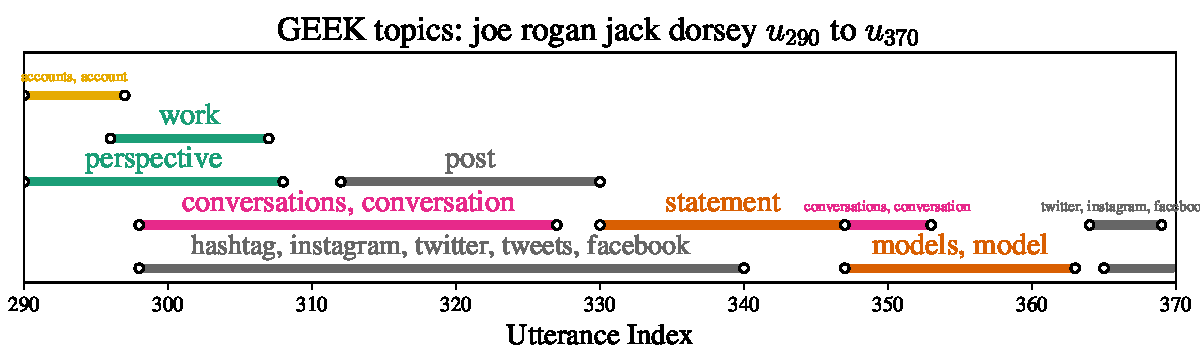
\includegraphics[width=\textwidth]{joe_rogan_jack_dorsey290_370_topics.pdf}
            \caption{The extracted topics within an excerpt of a conversation between podcast host Joe Rogan and twitter CEO Jack Dorsey. The y-axis is used to display simultaneous topics. Similar \glspl{keyphrase} are grouped together into topics. Topics are colour-coded by mapping \glspl{embedding} to a colour.}
            \label{fig:GEEK final result}
        \end{figure}

    \subsection{Evaluation}

    \subsubsection{Segmentation}
        Even though segmentation is not exactly possible as there are multiple topics that may overlap, by simply placing a topic boundary at the start of the largest topic out of a group of overlapping topics, we can achieve a reasonable approximation. This is visualised in Fig. \ref{fig:GEEK segment}.
        \begin{figure}
             \centering
             \begin{subfigure}[b]{\textwidth}
                 \centering
                 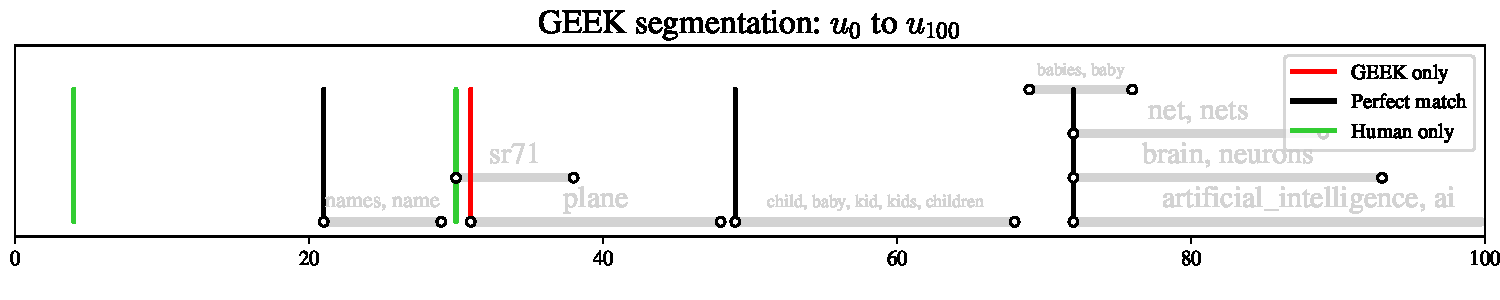
\includegraphics[width=1\textwidth]{figures/0to100segment_topics.pdf}
                 \caption{$u_0$ to $u_{100}$}
             \end{subfigure}
             \hfill
             \begin{subfigure}[b]{\textwidth}
                 \centering
                 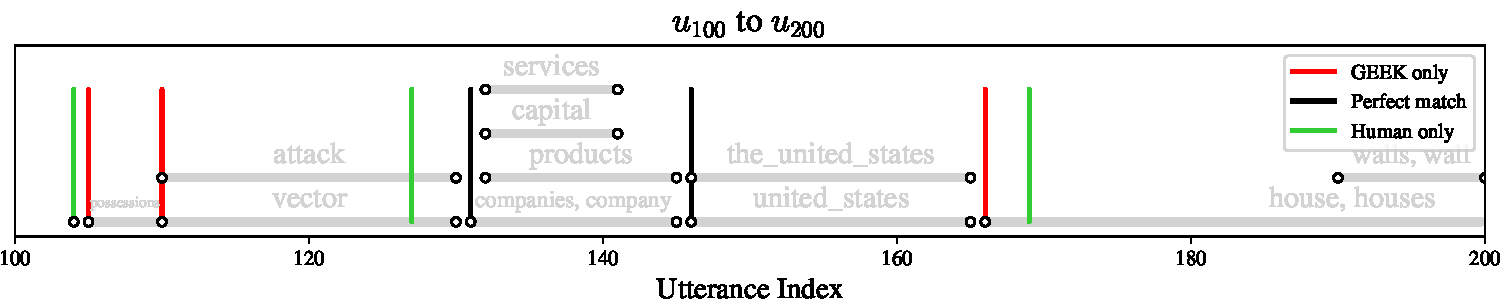
\includegraphics[width=1\textwidth]{figures/100to200segment_topics.pdf}
             \end{subfigure}
                \caption{200 \glspl{utterance} out of the evaluation transcript of a conversation between host Joe Rogan and guest Elon Musk. Vertical lines indicate boundaries: Green lines indicate human boundaries, red lines indicate boundaries placed by \gls{geek} and black lines are boundaries where the two agree exactly. Most boundaries are exactly or approximately detected by \gls{geek}. Failures include $u_4$ (missed topic change) or $u_{110}$ (false boundary).}
                \label{fig:GEEK segment}
        \end{figure}

        Using this approximation, \gls{geek} achieves a state of the art windowDiff score of
        \begin{equation}
            w_d = 0.22 \pm 0.04.
        \end{equation}


    \subsubsection{Labelling}
        We evaluate extracted topic labels in the same way we evaluated TopicRank \glspl{keyphrase} (Sec. \ref{method: topic rank}), with the small modification that multi-word topics match if any constituent words match the human annotation. This modification is small because multi-word topics already contain very similar words. \gls{geek} achieves an accuracy of
        \begin{equation}
            0.72 \pm 0.12,
        \end{equation}
        which is a significant improvement over TopicRank (see Eq. \ref{eq: topic rank accuracy}). It should be noted that only one author annotated selected \glspl{keyphrase}, which is a subjective task. It is expected that \gls{geek}'s accuracy is thus somewhat biased as its assumptions align more with the author's assumptions than TopicRanks's do. In future work it would be preferable to have multiple human annotators which provides an insight into labelling uncertainty and provides a more objective evaluation.

    \subsection{Limitations}
    \gls{geek} still suffers from some limitations, that we briefly outline here.

    \subsubsection{False Keywords}
        Some words are nouns and are used in conversation but do not describe topics. While \gls{geek} is somewhat robust against this, by requiring \glspl{keyphrase} to appear at least twice at least $T_{\text{min}}$ \glspl{utterance} apart, sometimes it fails. An example is the phrase ``attack vector" that Elon Musk uses in the conversation shown in Fig. \ref{fig:GEEK segment}. This phrase is a non-standard way of saying ``point of weakness", but because Elon Musk, and eventually the host Joe Rogan, keep using it, it is detected by \gls{geek} as two \glspl{keyphrase} ``attack" and ``vector". This leads to a wrong segmentation (the red vertical line at $u_{110})$.

    \subsubsection{Missed Topics}
        In some cases \gls{geek} also suffers from the opposite issue: minimum topic length may discard some actual topics that happen to be over quickly. An example for that is a missed boundary at $u_4$ in Fig. \ref{fig:GEEK segment}.

    \subsubsection{Ambiguous Embeddings}
        Certain matches are not detected because words can not be disambiguated (see Sec. \ref{fig:ambiguous_embedding}). For example, in Fig. \ref{fig:GEEK final result}, the \gls{keyphrase} ``post" should be included in the topic ``hasthag, instagram twitter, tweets, facebook", because ``post" and ``tweets" should be considered similar. Unfortunately, the word ``post" has ambiguous meanings, which leads to a poor embedding. To fix this, newer transformer \glspl{embedding} such as ElMo\cite{peters2018elmo} or BERT\cite{devlin2018bert}, that make \glspl{embedding} context-dependent and thus disambiguated could be evaluated in future work. \newline

\glsresetall % 2900 words
{\let\clearpage\relax \chapter[Annotated Corpus]{Corpus of Annotated Conversations}}

We apply our improved \gls{da} classification and topic extraction methods to 18,000 conversations randomly selected from the Spotify podcast corpus\cite{clifton-2020100000}. By annotating the transcript with the extracted linguistic features.

\section{Selection of Podcasts}
We select only podcasts with more than one speaker and of a minimum length of 100 \glspl{utterance}.

\section{Computational Optimisation}
We optimise our annotation of transcripts by caching language \glspl{model} and intermediate results such as inter-\gls{keyphrase} similarity in our topic extraction algorithm \gls{geek}.
We make the processing of transcripts multi-threaded and split the work-load between the graphical processing unit (GPU) and the central processing unit (CPU), because the graphical memory available for the GPU is limited and the cached \glspl{model} are large. This allows us to process three transcripts at once, at an average rate of $\approx 0.2$ transcripts/second leading to a total processing time of $\approx 25$ hours.

We are confident our implementation can not be optimised much further because more than $96\%$ of the computation times is used by the libraries we use (deep learning library keras CITE for \gls{da} classification and \gls{nlp} library flairNLP\cite{flairNLP}), and our system uses all available memory to store essential components.

\section{Access to Corpus}

As the Spotify podcast data-set requires approval for access, we can only provide our annotated corpus to researchers who have already been approved for said data-set. \newline

\chapter{Conclusions}
We aimed to evaluate a wide range of natural language processing techniques for dialogue act and topic analysis within the context of conversations and to improve them and we succeeded in doing so.
\subsubsection{State of the Art Dialogue Act Classification}
    For dialogue act classification, we select a 2017 model by Kumar et al., re-implement it within a newer python framework, fix an important bug and modernise components such as the word embeddings and recurrent neural network architecture, improving it from an accuracy of $79.2 \pm 0.3\%$ in the \gls{swda} Corpus to an accuracy of $84.6 \pm 0.3\%$, beating the previous state of the art accuracy of $83.1$ as well as the inter-annotator agreement accuracy of $84\%$ between the annotators who created the corpus.

\subsubsection{State of the Art Conversation Topic Modelling}
    Within the area of topic modelling, specifically when applying it to conversations, research is much less active than within dialogue act classification, and no standard corpora exist for evaluation. Therefore, we hand-annotated 4 podcast transcript excerpts and evaluated models against those. We evaluated it and other methods, such as utterance embedding based clustering, via a minimum-cut graph following the work of Malioutov et al., and other unsupervised clustering methods, but qualitatively achieve such underwhelming results that we do not attempt a quantitative evaluation. The previous state of the art topic-model, BayesSeg, performs better, but still does not achieve satisfactory performance, a \textit{windowDiff} penalty score of $0.39 \pm 0.06$ for topic segmentation.
    By identifying the key problem in all these approaches, the fact that many words in conversations are unrelated to the topic and therefore dilute seperation of dissimilar topics, we develop our own method: a graph of embedded extracted keyphrases (GEEK).
    GEEK follows a modified version of the TopicRank approach by Bougouin et al. to extract key-words and multi-word phrases that are likely to represent topics and then uses word embeddings of these key-words to identify semantically cohesive sections as topics with their keywords as topic labels. We find that GEEK is significantly more robust against weak key-word candidates than TopicRank by using semantically similar words to determine importance of candidates, not just repetitions of the exact candidate, and by filtering a list of 89 manually determined ``false flag" key-word candidates. We also improve the overall selection of keyphrases over TopicRank by employing named entity recognition to extract named entities (such as ``Donald Trump" or ``CIA"), which often indicate topics. Quantitatively, GEEK significantly improves upon the state of the art topic segmentation by BayesSeg, achieving the much lower \textit{windowDiff} penalty score of $\mathbf{0.22 \pm 0.04}$. We emphasize that this score is likely somewhat biased because we both \textit{created} the segmentation algorithm and annotated the dataset with which it is \textit{evaluated}, both of which are subject to our own biases as to what constitutes a topic and what constitutes a change of topic. However, we are confident that GEEK would still outperform the previous state of the art in an independently annotated dataset and propose the creation of such a dataset as a standardised metric to encourage and legitimise future work in this area.

\subsubsection{Creation of a Public Corpus of Annotated Podcast Transcripts}
    We parallelise and optimise our analysis methods to annotate a large selection of 18000 podcasts from the Spotify podcast corpus\cite{clifton-2020100000} with dialogue acts, keywords and topics. This corpus can be used to study a wide range of linguistic questions, such as \dots. Upon request, we make it available to any researchers that have also been granted access to the Spotify podcast corpus.
\glsresetall

\newpage % 800 words

%TC:ignore

\renewcommand{\headrulewidth}{0pt}% Remove header rule in bibliography
\pagestyle{plain}
\Urlmuskip=0mu plus 1mu
\emergencystretch=1em

\printbibliography
%TC:endignore
\end{document}
